\documentclass[english]{beamer}

\usepackage{amssymb}
\usepackage[]{babel}
\usepackage[]{amsmath}
\usepackage{xparse}
%\usepackage[colorlinks=true,linkcolor=blue,pdfborder={0 0 0}]{hyperref}
%\usepackage{microtype}
\usepackage{amsthm}
\usepackage{mathtools}
%\usepackage{todonotes}

\usepackage{chemformula}
\usepackage[exponent-product = \cdot]{siunitx}
\usepackage{booktabs}

\usetheme{Madrid}
\setbeamertemplate{bibliography item}[text]

\usepackage{fontspec}
\setmainfont{Linux Libertine O}
\setsansfont{Linux Biolinum O}
\usepackage{xcolor}

\usepackage[backend=biber,url=false]{biblatex}
\addbibresource{Vortrag.bib}

\graphicspath{ {images/} }

\title[Improvement of a \ch{NO} converter]{Further improvement of a \ch{NO}
  to \ch{NO2} converter for CE-DOAS measurements}
\subtitle{Bachelor thesis}
\institute[]{Institute of Environmental Physics\\Heidelberg University}
\author{Tim Adler}
\date{May 23, 2016}

\makeatletter
\hypersetup{
  pdftitle={\@title},
  pdfauthor={\@author},
}
\makeatother

\begin{document}

\begin{frame}
  \titlepage
  \begin{figure}[htbp]
    \centering
    
\includegraphics[width=0.2\textwidth]{images/unilogo.png}
    \hspace{1.5cm}
    
\includegraphics[width=0.2\textwidth]{images/LogoIUP.eps}
  \end{figure}
\end{frame}

\section{Motivation}

\begin{frame}
  \frametitle{Motivation}

  \begin{figure}[htbp]
    \centering
    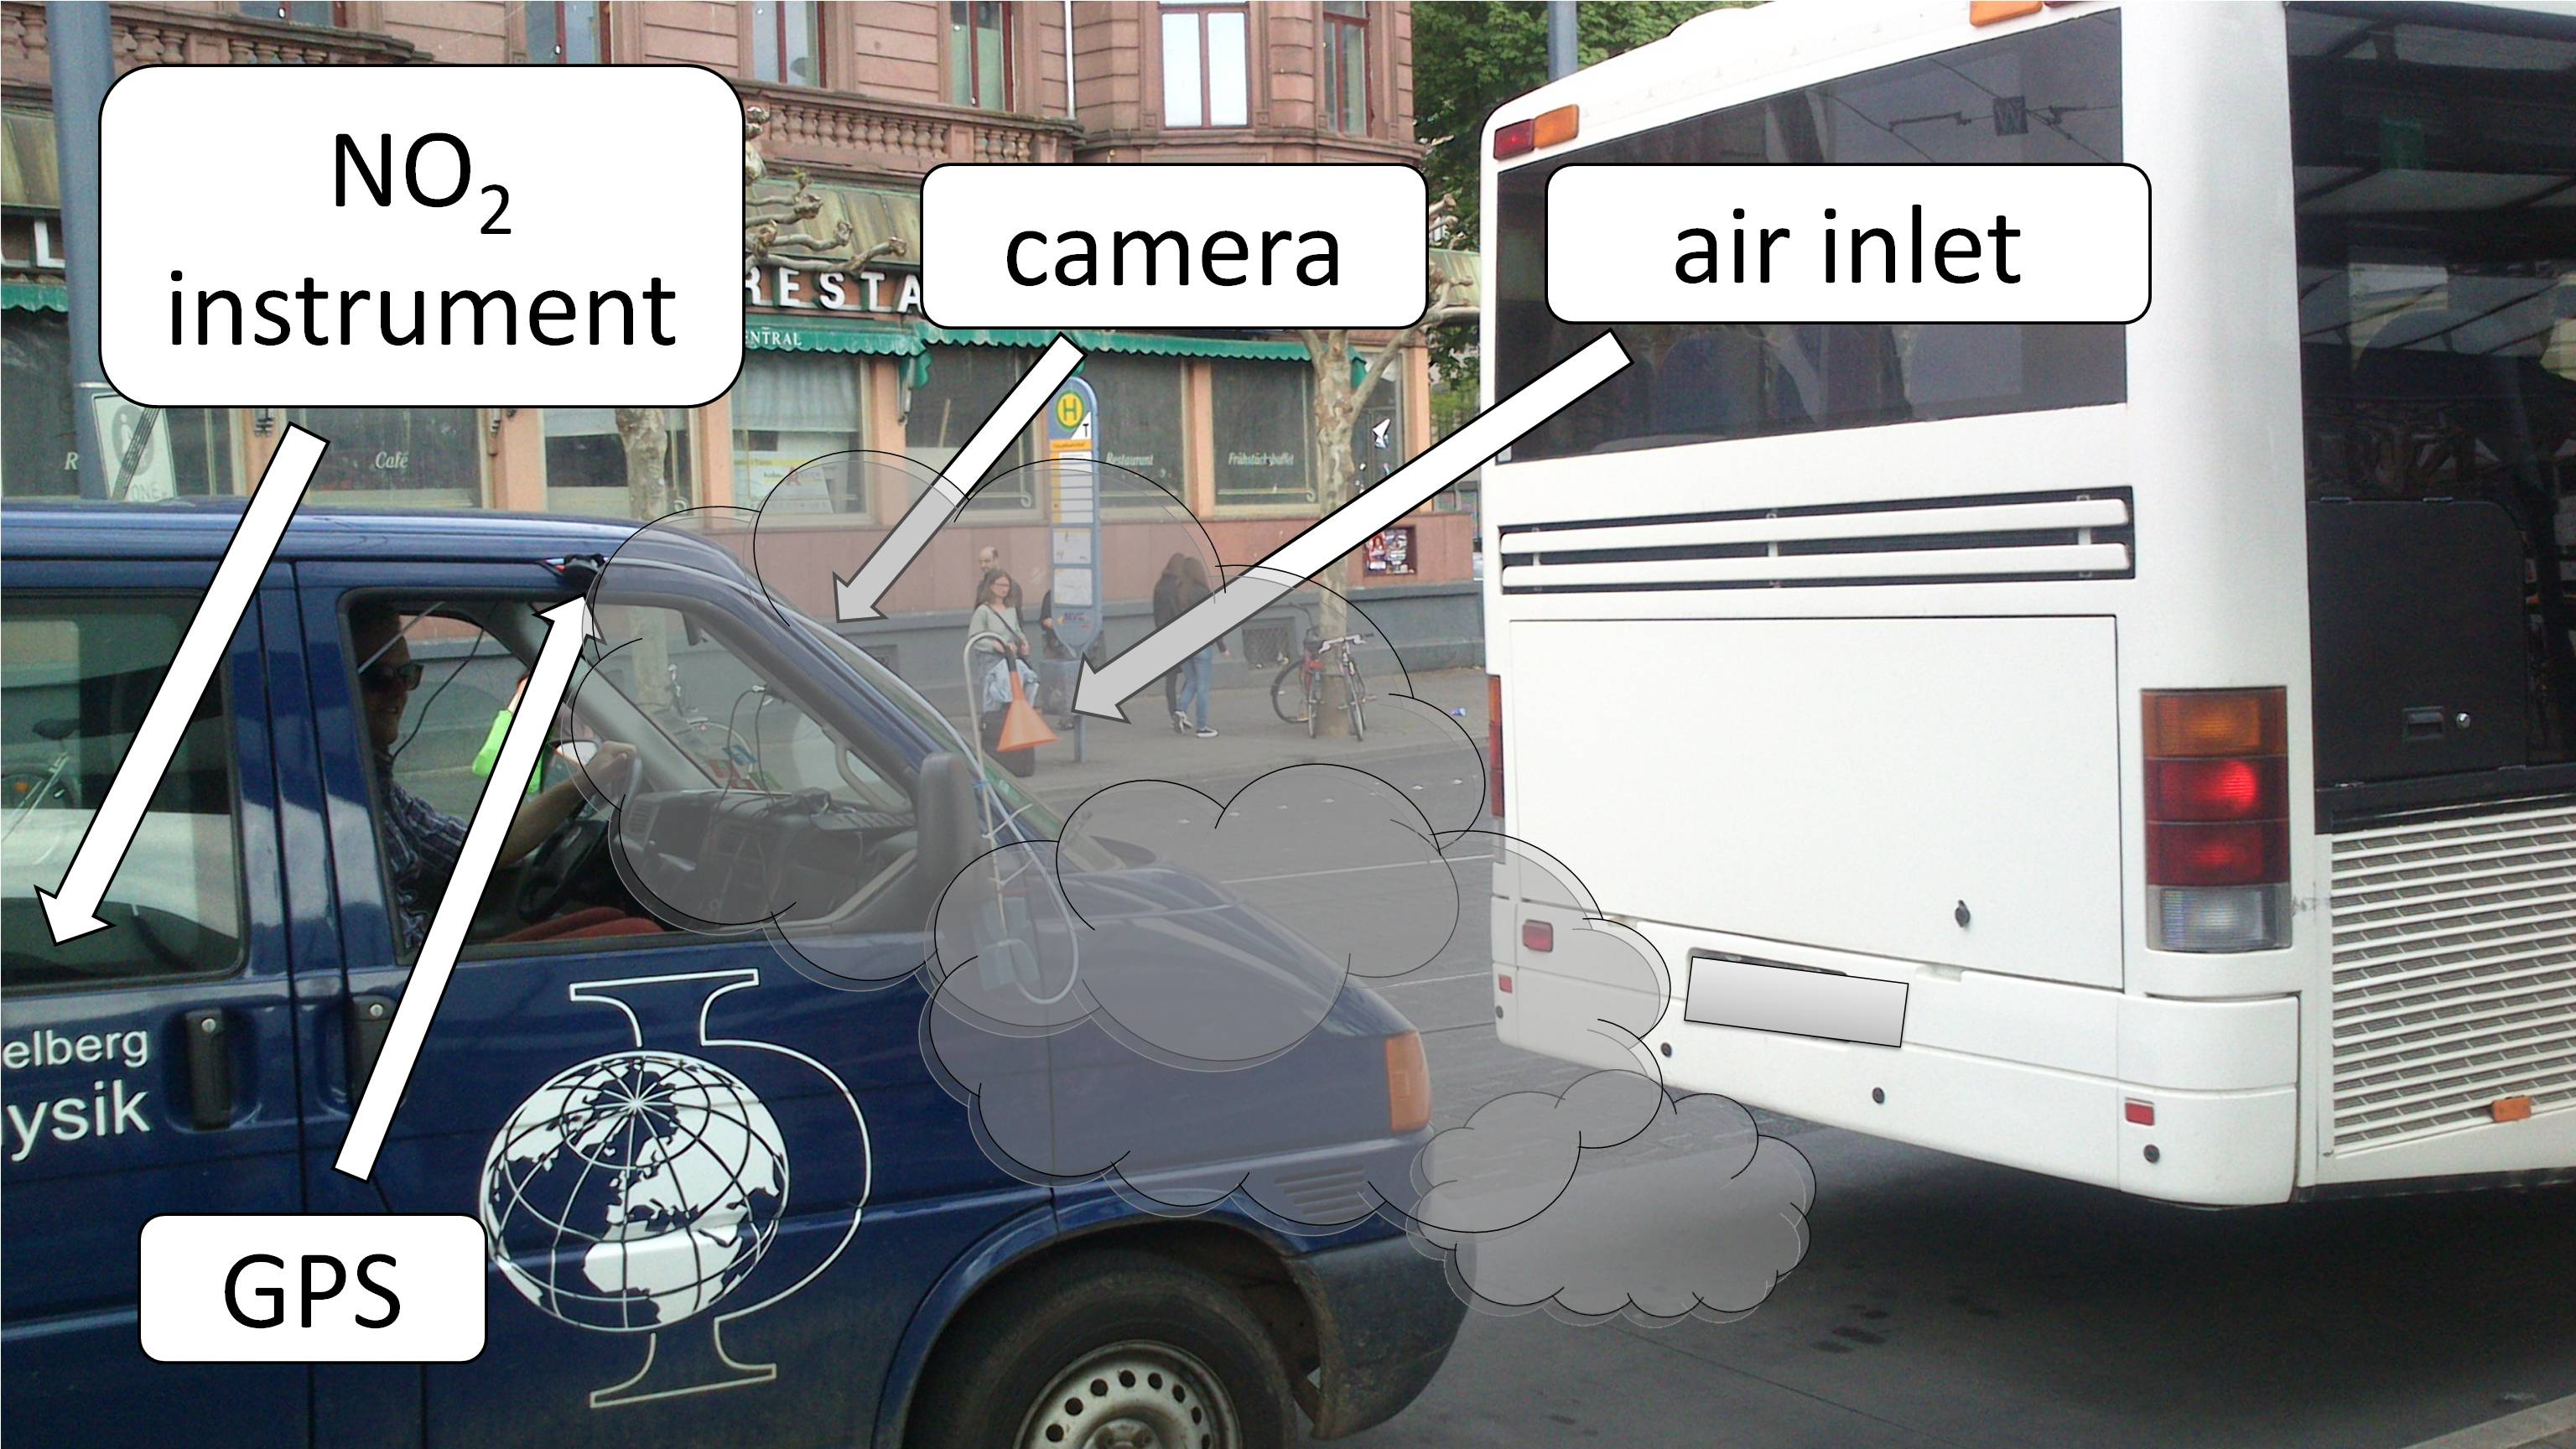
\includegraphics[width=0.55\textwidth]{vehicle_principle.jpg}
    \caption{Provided by \cite{denis}}
  \end{figure}

  \begin{itemize}
  \item In EU standards: \ch{NO_x\,=\ NO + NO2}
  \item \ch{NO} adsorption in deep UV
    \begin{itemize}
    \item No optical components
    \end{itemize}
  \item Solution: Indirect measurement
  \end{itemize}
\end{frame}

\begin{frame}
  \frametitle{Overview}
  \tableofcontents
\end{frame}

\section{Theory}

\begin{frame}
  \frametitle{Theory}
  \framesubtitle{Nitrogen monoxide conversion}
  \begin{itemize}
  \item Desired reaction:
    \begin{align*}
      \ch{NO + O3 & -> NO2 + O2}\\
      \intertext{\item Side effects:}
      \ch{NO2 + O3 & -> NO3 + O2}\\
      \ch{NO + NO3 & -> 2 NO2}\\
      \ch{NO2 + NO3 + M & <=> N2O5 + M}
    \end{align*}
  \end{itemize}
  
\end{frame}


\begin{frame}
  \frametitle{Theory}
  \framesubtitle{Ozone generation}
  \begin{itemize}
  \item Generation:
    \begin{align*}
      \ch{O2 + h}\nu &\ch{-> 2 O(^3P)} && \lambda < \SI{240}{\nano\meter}\\
      \ch{O(^3 P) + O2 + M} &\ch{-> O3 + M}\\
      \intertext{\item Dissociation:}
      \ch{O3 + h}\nu \ch{&-> O(^1 D) + O2} && \lambda < \SI{310}{\nano\meter}\\
      \ch{O(^1 D) + M & -> O(^3 P) + M}\\
      \intertext{\item Destruction:}
      \ch{O(^3 P) + O3 & -> 2 O2}
    \end{align*}
  \end{itemize}
\end{frame}

\begin{frame}
  \frametitle{Theory} \framesubtitle{Ozone generation}
  \begin{figure}[htbp] \centering
    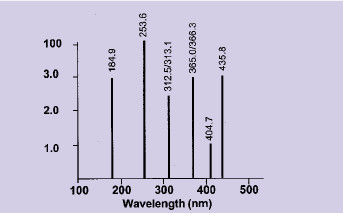
\includegraphics[]{hg.jpg}
    \caption{Spectrum of the Pen-Ray mercury lamp. The plot was taken
      out of~\cite{lamp}.}
    \label{fig:hg}
  \end{figure}
\end{frame}

\begin{frame}
  \frametitle{Theory}
  \framesubtitle{Laughing gas conversion}
  \begin{itemize}
  \item Primary decay reaction:
    \begin{align*}
      \ch{N2O + h}\nu \ch{& -> N2 + O(^1 D)} && \SI{185}{\nano\meter}
                                                \leq \lambda \leq
                         \SI{230}{\nano\meter}\\
      \intertext{\item Secondary decay reactions:}
      \ch{N2O + O(^1 D) & -> 2 NO}\\
      \ch{N2O + O(^1 D) & -> N2 + O2}
    \end{align*}
  \item \ch{N2O} passes filter barriers
    \begin{itemize}
    \item Filter \ch{NO}/\ch{NO2} after conversion
    \item Silica suitable as \ch{O3} can pass
    \end{itemize}
  \end{itemize}
\end{frame}

\begin{frame}
  \frametitle{Theory}
  \framesubtitle{CE-DOAS}
  \begin{itemize}
  \item Absorption spectroscopy
    \begin{itemize}
    \item Lambert-Beer law
    \end{itemize}

  \item Comparison of \(I_0\) and \(I\)
  \end{itemize}
  \begin{figure}[htbp]
    \centering
    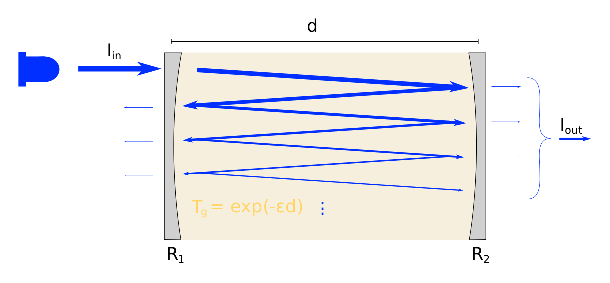
\includegraphics[scale=.5]{images/reflection.eps}
    \caption{Simplified schematic overview of a cavity.}
    \label{fig:cavity}
  \end{figure}
  \begin{align*}
    I_{\text{out}} = I_{\text{in}} \cdot \frac{T_1 T_2 T_g}{1 - R_1 R_2 {T_g}^2}
  \end{align*}
\end{frame}


\begin{frame}
  \frametitle{Theory}
  \framesubtitle{CE-DOAS}
  
  The central equations for the evaluation are:

  \begin{align*}
    D_{CE} & = \ln\left(\frac{I_0}{I}\right) \stackrel{!}{=}
             L_{\text{eff}} \cdot \left (\sum_i \sigma_i \cdot c_i
             + \Delta \varepsilon_{\text{Rayleigh}} \right)\\
    L_{\text{eff}} &  = \frac{D_{CE}}{\exp(D_{CE}) - 1} \cdot L_0 \\
    L_0 & = \frac{d}{1 - R + d\varepsilon_0}\\
    \frac{I_0}{I} & = 1 +  L_0 \cdot \left (\sum_i \sigma_i \cdot c_i
             + \Delta \varepsilon_{\text{Rayleigh}} \right)
  \end{align*}
  % \begin{description}
  % \item[\(D_{CE}\):] Cavity enhanced optical density
  % \item[\(L_{\text{eff}}\):] Effective pathlength
  % \item[\(L_0\):] Vacuum pathlength
  % \end{description}
\end{frame}

\section{Setup}

\begin{frame}
  \frametitle{Setup}
  \begin{figure}[htbp]
    \centering
    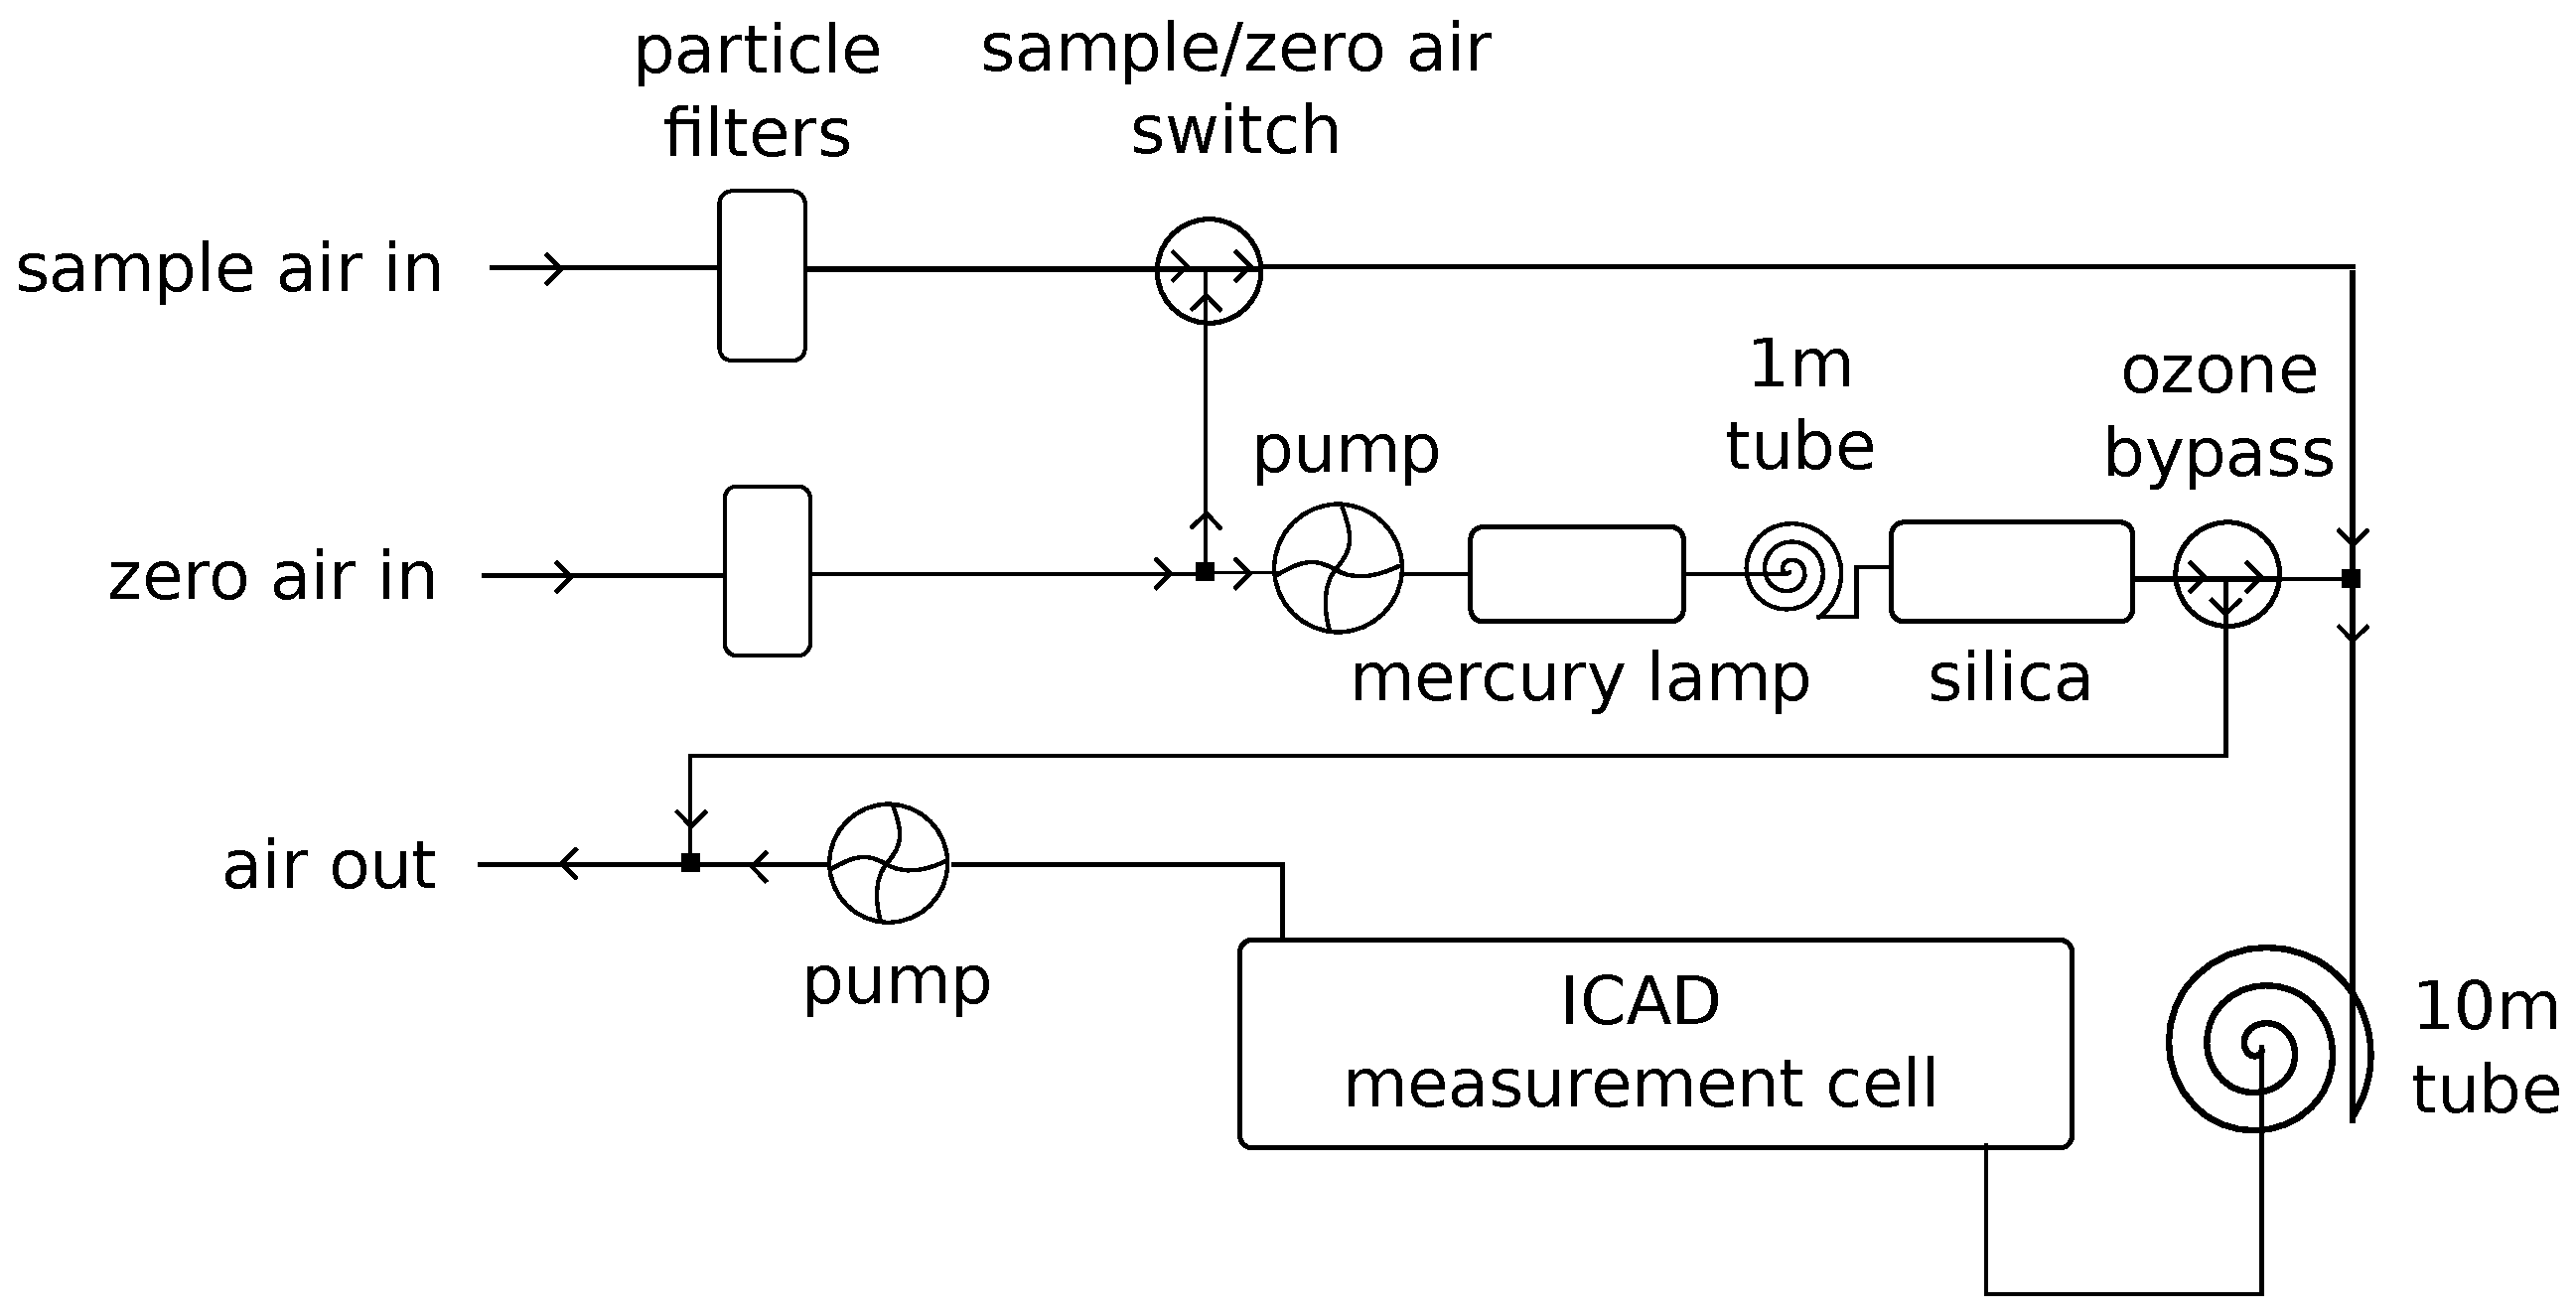
\includegraphics[width=0.7\textwidth]{images/envimes_setup.eps}
    \caption{Measurement setup}
    \label{fig:setup}
  \end{figure}
\end{frame}

\begin{frame}
  \frametitle{Setup}
  \begin{figure}[htbp]
    \centering
    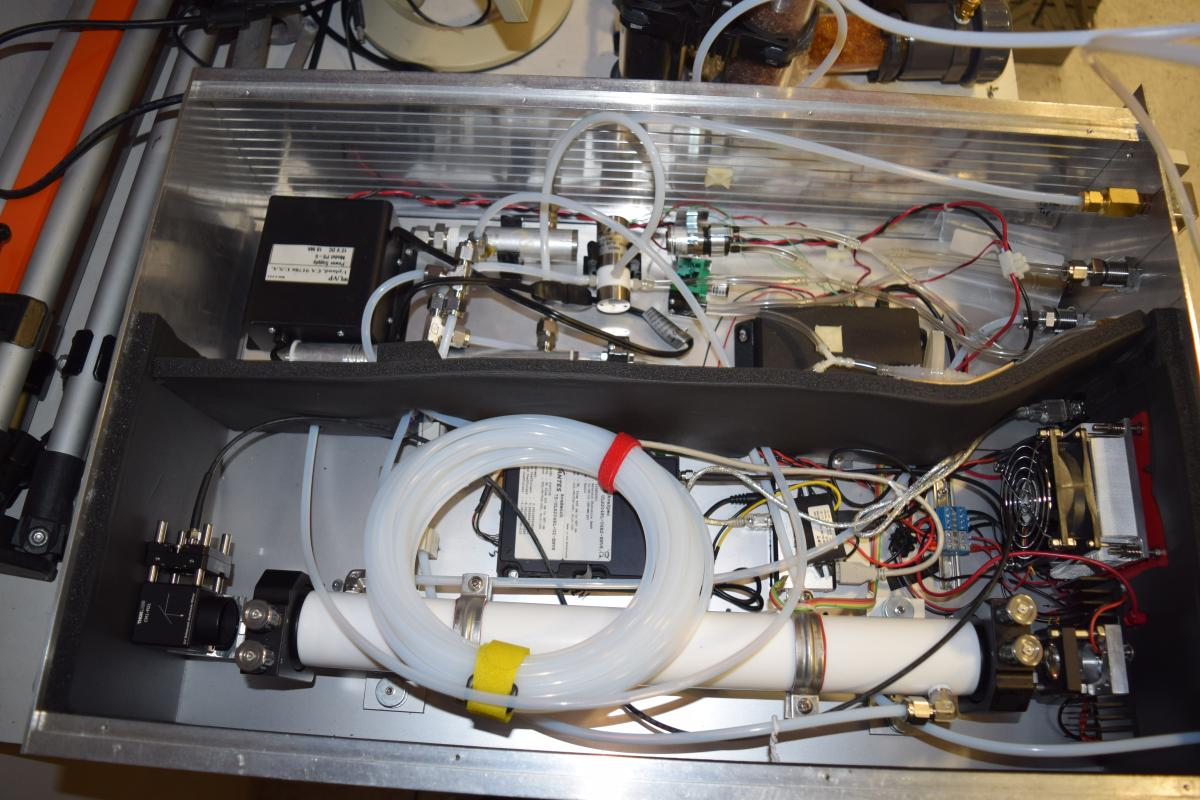
\includegraphics[width=0.7\textwidth]{images/envimes_up.jpg}
    \caption{Measurement setup}
    \label{fig:setup}
  \end{figure}
\end{frame}


\section{Measurements}

\begin{frame}
  \frametitle{Measurements}
  \framesubtitle{\ch{NO2} contamination of \ch{O3} enriched air}
  \begin{figure}[htbp]
    \centering
    \scalebox{.7}{
      % GNUPLOT: LaTeX picture with Postscript
\begingroup
  \makeatletter
  \providecommand\color[2][]{%
    \GenericError{(gnuplot) \space\space\space\@spaces}{%
      Package color not loaded in conjunction with
      terminal option `colourtext'%
    }{See the gnuplot documentation for explanation.%
    }{Either use 'blacktext' in gnuplot or load the package
      color.sty in LaTeX.}%
    \renewcommand\color[2][]{}%
  }%
  \providecommand\includegraphics[2][]{%
    \GenericError{(gnuplot) \space\space\space\@spaces}{%
      Package graphicx or graphics not loaded%
    }{See the gnuplot documentation for explanation.%
    }{The gnuplot epslatex terminal needs graphicx.sty or graphics.sty.}%
    \renewcommand\includegraphics[2][]{}%
  }%
  \providecommand\rotatebox[2]{#2}%
  \@ifundefined{ifGPcolor}{%
    \newif\ifGPcolor
    \GPcolorfalse
  }{}%
  \@ifundefined{ifGPblacktext}{%
    \newif\ifGPblacktext
    \GPblacktexttrue
  }{}%
  % define a \g@addto@macro without @ in the name:
  \let\gplgaddtomacro\g@addto@macro
  % define empty templates for all commands taking text:
  \gdef\gplbacktext{}%
  \gdef\gplfronttext{}%
  \makeatother
  \ifGPblacktext
    % no textcolor at all
    \def\colorrgb#1{}%
    \def\colorgray#1{}%
  \else
    % gray or color?
    \ifGPcolor
      \def\colorrgb#1{\color[rgb]{#1}}%
      \def\colorgray#1{\color[gray]{#1}}%
      \expandafter\def\csname LTw\endcsname{\color{white}}%
      \expandafter\def\csname LTb\endcsname{\color{black}}%
      \expandafter\def\csname LTa\endcsname{\color{black}}%
      \expandafter\def\csname LT0\endcsname{\color[rgb]{1,0,0}}%
      \expandafter\def\csname LT1\endcsname{\color[rgb]{0,1,0}}%
      \expandafter\def\csname LT2\endcsname{\color[rgb]{0,0,1}}%
      \expandafter\def\csname LT3\endcsname{\color[rgb]{1,0,1}}%
      \expandafter\def\csname LT4\endcsname{\color[rgb]{0,1,1}}%
      \expandafter\def\csname LT5\endcsname{\color[rgb]{1,1,0}}%
      \expandafter\def\csname LT6\endcsname{\color[rgb]{0,0,0}}%
      \expandafter\def\csname LT7\endcsname{\color[rgb]{1,0.3,0}}%
      \expandafter\def\csname LT8\endcsname{\color[rgb]{0.5,0.5,0.5}}%
    \else
      % gray
      \def\colorrgb#1{\color{black}}%
      \def\colorgray#1{\color[gray]{#1}}%
      \expandafter\def\csname LTw\endcsname{\color{white}}%
      \expandafter\def\csname LTb\endcsname{\color{black}}%
      \expandafter\def\csname LTa\endcsname{\color{black}}%
      \expandafter\def\csname LT0\endcsname{\color{black}}%
      \expandafter\def\csname LT1\endcsname{\color{black}}%
      \expandafter\def\csname LT2\endcsname{\color{black}}%
      \expandafter\def\csname LT3\endcsname{\color{black}}%
      \expandafter\def\csname LT4\endcsname{\color{black}}%
      \expandafter\def\csname LT5\endcsname{\color{black}}%
      \expandafter\def\csname LT6\endcsname{\color{black}}%
      \expandafter\def\csname LT7\endcsname{\color{black}}%
      \expandafter\def\csname LT8\endcsname{\color{black}}%
    \fi
  \fi
    \setlength{\unitlength}{0.0500bp}%
    \ifx\gptboxheight\undefined%
      \newlength{\gptboxheight}%
      \newlength{\gptboxwidth}%
      \newsavebox{\gptboxtext}%
    \fi%
    \setlength{\fboxrule}{0.5pt}%
    \setlength{\fboxsep}{1pt}%
\begin{picture}(3888.00,3888.00)%
    \gplgaddtomacro\gplbacktext{%
      \csname LTb\endcsname%
      \put(682,862){\makebox(0,0)[r]{\strut{}$0$}}%
      \put(682,1177){\makebox(0,0)[r]{\strut{}$2$}}%
      \put(682,1492){\makebox(0,0)[r]{\strut{}$4$}}%
      \put(682,1808){\makebox(0,0)[r]{\strut{}$6$}}%
      \put(682,2123){\makebox(0,0)[r]{\strut{}$8$}}%
      \put(682,2439){\makebox(0,0)[r]{\strut{}$10$}}%
      \put(682,2754){\makebox(0,0)[r]{\strut{}$12$}}%
      \put(682,3069){\makebox(0,0)[r]{\strut{}$14$}}%
      \put(814,484){\makebox(0,0){\strut{}$0$}}%
      \put(1196,484){\makebox(0,0){\strut{}$0.05$}}%
      \put(1579,484){\makebox(0,0){\strut{}$0.1$}}%
      \put(1961,484){\makebox(0,0){\strut{}$0.15$}}%
      \put(2344,484){\makebox(0,0){\strut{}$0.2$}}%
      \put(2726,484){\makebox(0,0){\strut{}$0.25$}}%
      \put(3109,484){\makebox(0,0){\strut{}$0.3$}}%
      \put(3491,484){\makebox(0,0){\strut{}$0.35$}}%
    }%
    \gplgaddtomacro\gplfronttext{%
      \csname LTb\endcsname%
      \put(176,1965){\rotatebox{-270}{\makebox(0,0){\strut{}Concentration [ppb]}}}%
      \put(2152,154){\makebox(0,0){\strut{}Flow [\si{\liter\per\minute}]}}%
      \put(2152,3557){\makebox(0,0){\strut{}Nitrogen Dioxide}}%
      \csname LTb\endcsname%
      \put(2504,2185){\makebox(0,0)[r]{\strut{}f,  i}}%
      \csname LTb\endcsname%
      \put(2504,1965){\makebox(0,0)[r]{\strut{}f, d}}%
      \csname LTb\endcsname%
      \put(2504,1745){\makebox(0,0)[r]{\strut{}nf, i}}%
    }%
    \gplbacktext
    \put(0,0){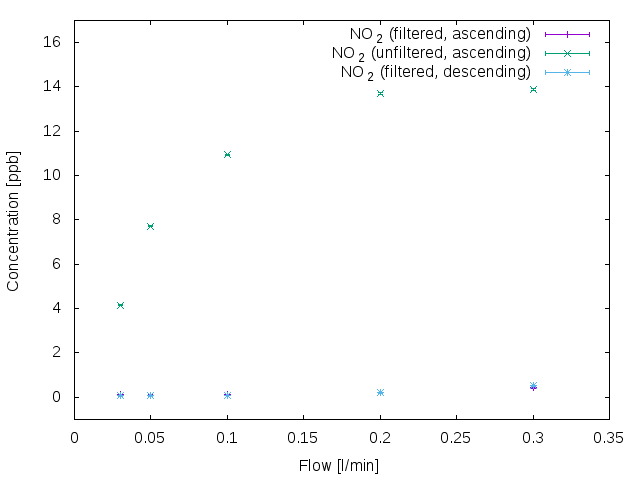
\includegraphics{../images/NO2}}%
    \gplfronttext
  \end{picture}%
\endgroup

    }
    \hspace{1cm}
    \scalebox{.7}{
      % GNUPLOT: LaTeX picture with Postscript
\begingroup
  \makeatletter
  \providecommand\color[2][]{%
    \GenericError{(gnuplot) \space\space\space\@spaces}{%
      Package color not loaded in conjunction with
      terminal option `colourtext'%
    }{See the gnuplot documentation for explanation.%
    }{Either use 'blacktext' in gnuplot or load the package
      color.sty in LaTeX.}%
    \renewcommand\color[2][]{}%
  }%
  \providecommand\includegraphics[2][]{%
    \GenericError{(gnuplot) \space\space\space\@spaces}{%
      Package graphicx or graphics not loaded%
    }{See the gnuplot documentation for explanation.%
    }{The gnuplot epslatex terminal needs graphicx.sty or graphics.sty.}%
    \renewcommand\includegraphics[2][]{}%
  }%
  \providecommand\rotatebox[2]{#2}%
  \@ifundefined{ifGPcolor}{%
    \newif\ifGPcolor
    \GPcolorfalse
  }{}%
  \@ifundefined{ifGPblacktext}{%
    \newif\ifGPblacktext
    \GPblacktexttrue
  }{}%
  % define a \g@addto@macro without @ in the name:
  \let\gplgaddtomacro\g@addto@macro
  % define empty templates for all commands taking text:
  \gdef\gplbacktext{}%
  \gdef\gplfronttext{}%
  \makeatother
  \ifGPblacktext
    % no textcolor at all
    \def\colorrgb#1{}%
    \def\colorgray#1{}%
  \else
    % gray or color?
    \ifGPcolor
      \def\colorrgb#1{\color[rgb]{#1}}%
      \def\colorgray#1{\color[gray]{#1}}%
      \expandafter\def\csname LTw\endcsname{\color{white}}%
      \expandafter\def\csname LTb\endcsname{\color{black}}%
      \expandafter\def\csname LTa\endcsname{\color{black}}%
      \expandafter\def\csname LT0\endcsname{\color[rgb]{1,0,0}}%
      \expandafter\def\csname LT1\endcsname{\color[rgb]{0,1,0}}%
      \expandafter\def\csname LT2\endcsname{\color[rgb]{0,0,1}}%
      \expandafter\def\csname LT3\endcsname{\color[rgb]{1,0,1}}%
      \expandafter\def\csname LT4\endcsname{\color[rgb]{0,1,1}}%
      \expandafter\def\csname LT5\endcsname{\color[rgb]{1,1,0}}%
      \expandafter\def\csname LT6\endcsname{\color[rgb]{0,0,0}}%
      \expandafter\def\csname LT7\endcsname{\color[rgb]{1,0.3,0}}%
      \expandafter\def\csname LT8\endcsname{\color[rgb]{0.5,0.5,0.5}}%
    \else
      % gray
      \def\colorrgb#1{\color{black}}%
      \def\colorgray#1{\color[gray]{#1}}%
      \expandafter\def\csname LTw\endcsname{\color{white}}%
      \expandafter\def\csname LTb\endcsname{\color{black}}%
      \expandafter\def\csname LTa\endcsname{\color{black}}%
      \expandafter\def\csname LT0\endcsname{\color{black}}%
      \expandafter\def\csname LT1\endcsname{\color{black}}%
      \expandafter\def\csname LT2\endcsname{\color{black}}%
      \expandafter\def\csname LT3\endcsname{\color{black}}%
      \expandafter\def\csname LT4\endcsname{\color{black}}%
      \expandafter\def\csname LT5\endcsname{\color{black}}%
      \expandafter\def\csname LT6\endcsname{\color{black}}%
      \expandafter\def\csname LT7\endcsname{\color{black}}%
      \expandafter\def\csname LT8\endcsname{\color{black}}%
    \fi
  \fi
    \setlength{\unitlength}{0.0500bp}%
    \ifx\gptboxheight\undefined%
      \newlength{\gptboxheight}%
      \newlength{\gptboxwidth}%
      \newsavebox{\gptboxtext}%
    \fi%
    \setlength{\fboxrule}{0.5pt}%
    \setlength{\fboxsep}{1pt}%
\begin{picture}(4030.00,4030.00)%
    \gplgaddtomacro\gplbacktext{%
      \csname LTb\endcsname%
      \put(682,704){\makebox(0,0)[r]{\strut{}$2$}}%
      \put(682,1148){\makebox(0,0)[r]{\strut{}$4$}}%
      \put(682,1592){\makebox(0,0)[r]{\strut{}$6$}}%
      \put(682,2037){\makebox(0,0)[r]{\strut{}$8$}}%
      \put(682,2481){\makebox(0,0)[r]{\strut{}$10$}}%
      \put(682,2925){\makebox(0,0)[r]{\strut{}$12$}}%
      \put(682,3369){\makebox(0,0)[r]{\strut{}$14$}}%
      \put(814,484){\makebox(0,0){\strut{}$0$}}%
      \put(1217,484){\makebox(0,0){\strut{}$0.05$}}%
      \put(1619,484){\makebox(0,0){\strut{}$0.1$}}%
      \put(2022,484){\makebox(0,0){\strut{}$0.15$}}%
      \put(2425,484){\makebox(0,0){\strut{}$0.2$}}%
      \put(2828,484){\makebox(0,0){\strut{}$0.25$}}%
      \put(3230,484){\makebox(0,0){\strut{}$0.3$}}%
      \put(3633,484){\makebox(0,0){\strut{}$0.35$}}%
    }%
    \gplgaddtomacro\gplfronttext{%
      \csname LTb\endcsname%
      \put(176,2036){\rotatebox{-270}{\makebox(0,0){\strut{}Concentration [ppm]}}}%
      \put(2223,154){\makebox(0,0){\strut{}Flow [\si{\liter\per\minute}]}}%
      \put(2223,3699){\makebox(0,0){\strut{}Ozone}}%
    }%
    \gplbacktext
    \put(0,0){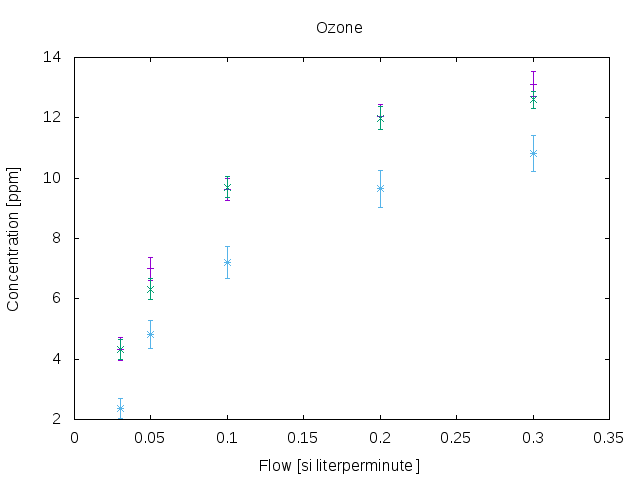
\includegraphics{../images/O3}}%
    \gplfronttext
  \end{picture}%
\endgroup

    }
    \caption{\ch{NO2} and \ch{O3} concentration at different flows
      with (f) and without (nf) the silica gel filter.}
    \label{fig:flow}
  \end{figure}
\end{frame}

\begin{frame}
  \frametitle{Measurements}
  \framesubtitle{Pure \ch{NO} measurements in synthetic air}
  \begin{figure}[htbp]
    \centering
    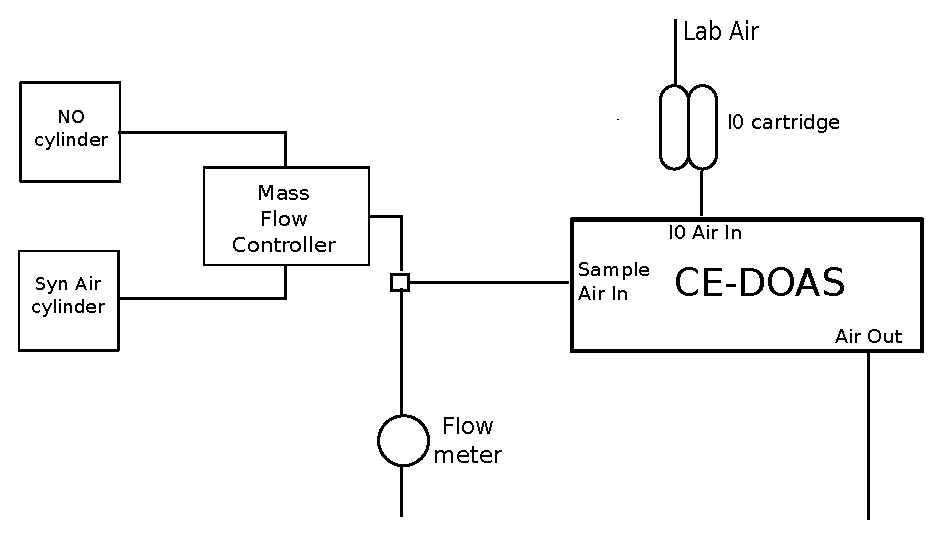
\includegraphics[width=0.6\textwidth]{no_setup.eps}
    \caption{Setup of the pure \ch{NO} measurement.}
    \label{fig:no-setup}
  \end{figure}
\end{frame}

\begin{frame}
  \frametitle{Measurements}
  \framesubtitle{Pure \ch{NO} measurements in synthetic air}
  \begin{figure}[htbp]
    \centering
    \scalebox{.7}{
      % GNUPLOT: LaTeX picture with Postscript
\begingroup
  \makeatletter
  \providecommand\color[2][]{%
    \GenericError{(gnuplot) \space\space\space\@spaces}{%
      Package color not loaded in conjunction with
      terminal option `colourtext'%
    }{See the gnuplot documentation for explanation.%
    }{Either use 'blacktext' in gnuplot or load the package
      color.sty in LaTeX.}%
    \renewcommand\color[2][]{}%
  }%
  \providecommand\includegraphics[2][]{%
    \GenericError{(gnuplot) \space\space\space\@spaces}{%
      Package graphicx or graphics not loaded%
    }{See the gnuplot documentation for explanation.%
    }{The gnuplot epslatex terminal needs graphicx.sty or graphics.sty.}%
    \renewcommand\includegraphics[2][]{}%
  }%
  \providecommand\rotatebox[2]{#2}%
  \@ifundefined{ifGPcolor}{%
    \newif\ifGPcolor
    \GPcolorfalse
  }{}%
  \@ifundefined{ifGPblacktext}{%
    \newif\ifGPblacktext
    \GPblacktexttrue
  }{}%
  % define a \g@addto@macro without @ in the name:
  \let\gplgaddtomacro\g@addto@macro
  % define empty templates for all commands taking text:
  \gdef\gplbacktext{}%
  \gdef\gplfronttext{}%
  \makeatother
  \ifGPblacktext
    % no textcolor at all
    \def\colorrgb#1{}%
    \def\colorgray#1{}%
  \else
    % gray or color?
    \ifGPcolor
      \def\colorrgb#1{\color[rgb]{#1}}%
      \def\colorgray#1{\color[gray]{#1}}%
      \expandafter\def\csname LTw\endcsname{\color{white}}%
      \expandafter\def\csname LTb\endcsname{\color{black}}%
      \expandafter\def\csname LTa\endcsname{\color{black}}%
      \expandafter\def\csname LT0\endcsname{\color[rgb]{1,0,0}}%
      \expandafter\def\csname LT1\endcsname{\color[rgb]{0,1,0}}%
      \expandafter\def\csname LT2\endcsname{\color[rgb]{0,0,1}}%
      \expandafter\def\csname LT3\endcsname{\color[rgb]{1,0,1}}%
      \expandafter\def\csname LT4\endcsname{\color[rgb]{0,1,1}}%
      \expandafter\def\csname LT5\endcsname{\color[rgb]{1,1,0}}%
      \expandafter\def\csname LT6\endcsname{\color[rgb]{0,0,0}}%
      \expandafter\def\csname LT7\endcsname{\color[rgb]{1,0.3,0}}%
      \expandafter\def\csname LT8\endcsname{\color[rgb]{0.5,0.5,0.5}}%
    \else
      % gray
      \def\colorrgb#1{\color{black}}%
      \def\colorgray#1{\color[gray]{#1}}%
      \expandafter\def\csname LTw\endcsname{\color{white}}%
      \expandafter\def\csname LTb\endcsname{\color{black}}%
      \expandafter\def\csname LTa\endcsname{\color{black}}%
      \expandafter\def\csname LT0\endcsname{\color{black}}%
      \expandafter\def\csname LT1\endcsname{\color{black}}%
      \expandafter\def\csname LT2\endcsname{\color{black}}%
      \expandafter\def\csname LT3\endcsname{\color{black}}%
      \expandafter\def\csname LT4\endcsname{\color{black}}%
      \expandafter\def\csname LT5\endcsname{\color{black}}%
      \expandafter\def\csname LT6\endcsname{\color{black}}%
      \expandafter\def\csname LT7\endcsname{\color{black}}%
      \expandafter\def\csname LT8\endcsname{\color{black}}%
    \fi
  \fi
    \setlength{\unitlength}{0.0500bp}%
    \ifx\gptboxheight\undefined%
      \newlength{\gptboxheight}%
      \newlength{\gptboxwidth}%
      \newsavebox{\gptboxtext}%
    \fi%
    \setlength{\fboxrule}{0.5pt}%
    \setlength{\fboxsep}{1pt}%
\begin{picture}(4030.00,4030.00)%
    \gplgaddtomacro\gplbacktext{%
      \csname LTb\endcsname%
      \put(682,686){\makebox(0,0)[r]{\strut{}$0$}}%
      \put(682,984){\makebox(0,0)[r]{\strut{}$10$}}%
      \put(682,1282){\makebox(0,0)[r]{\strut{}$20$}}%
      \put(682,1580){\makebox(0,0)[r]{\strut{}$30$}}%
      \put(682,1878){\makebox(0,0)[r]{\strut{}$40$}}%
      \put(682,2177){\makebox(0,0)[r]{\strut{}$50$}}%
      \put(682,2475){\makebox(0,0)[r]{\strut{}$60$}}%
      \put(682,2773){\makebox(0,0)[r]{\strut{}$70$}}%
      \put(682,3071){\makebox(0,0)[r]{\strut{}$80$}}%
      \put(682,3369){\makebox(0,0)[r]{\strut{}$90$}}%
      \put(814,554){\rotatebox{-45}{\makebox(0,0)[l]{\strut{}16:00}}}%
      \put(1096,554){\rotatebox{-45}{\makebox(0,0)[l]{\strut{}17:00}}}%
      \put(1378,554){\rotatebox{-45}{\makebox(0,0)[l]{\strut{}18:00}}}%
      \put(1660,554){\rotatebox{-45}{\makebox(0,0)[l]{\strut{}19:00}}}%
      \put(1942,554){\rotatebox{-45}{\makebox(0,0)[l]{\strut{}20:00}}}%
      \put(2224,554){\rotatebox{-45}{\makebox(0,0)[l]{\strut{}21:00}}}%
      \put(2505,554){\rotatebox{-45}{\makebox(0,0)[l]{\strut{}22:00}}}%
      \put(2787,554){\rotatebox{-45}{\makebox(0,0)[l]{\strut{}23:00}}}%
      \put(3069,554){\rotatebox{-45}{\makebox(0,0)[l]{\strut{}00:00}}}%
      \put(3351,554){\rotatebox{-45}{\makebox(0,0)[l]{\strut{}01:00}}}%
      \put(3633,554){\rotatebox{-45}{\makebox(0,0)[l]{\strut{}02:00}}}%
    }%
    \gplgaddtomacro\gplfronttext{%
      \csname LTb\endcsname%
      \put(176,2027){\rotatebox{-270}{\makebox(0,0){\strut{}Concentration [ppb]}}}%
      \put(2223,3699){\makebox(0,0){\strut{}Nitrogen Dioxide}}%
    }%
    \gplbacktext
    \put(0,0){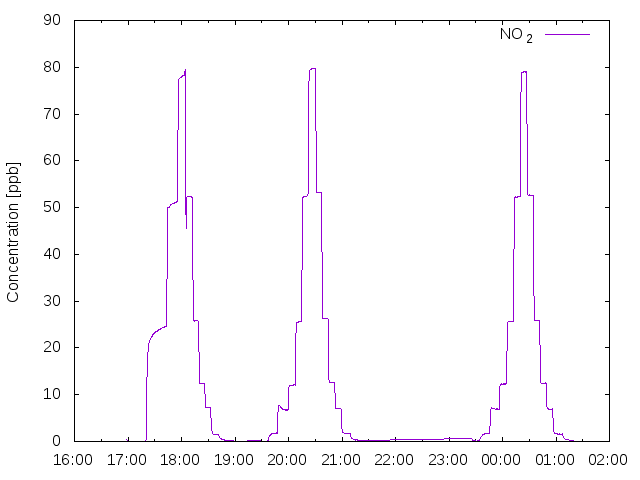
\includegraphics{../images/20160222_NO_fixI0_NO_ts}}%
    \gplfronttext
  \end{picture}%
\endgroup

    }
    \hspace{1cm}
    \scalebox{.7}{
      % GNUPLOT: LaTeX picture with Postscript
\begingroup
  \makeatletter
  \providecommand\color[2][]{%
    \GenericError{(gnuplot) \space\space\space\@spaces}{%
      Package color not loaded in conjunction with
      terminal option `colourtext'%
    }{See the gnuplot documentation for explanation.%
    }{Either use 'blacktext' in gnuplot or load the package
      color.sty in LaTeX.}%
    \renewcommand\color[2][]{}%
  }%
  \providecommand\includegraphics[2][]{%
    \GenericError{(gnuplot) \space\space\space\@spaces}{%
      Package graphicx or graphics not loaded%
    }{See the gnuplot documentation for explanation.%
    }{The gnuplot epslatex terminal needs graphicx.sty or graphics.sty.}%
    \renewcommand\includegraphics[2][]{}%
  }%
  \providecommand\rotatebox[2]{#2}%
  \@ifundefined{ifGPcolor}{%
    \newif\ifGPcolor
    \GPcolorfalse
  }{}%
  \@ifundefined{ifGPblacktext}{%
    \newif\ifGPblacktext
    \GPblacktexttrue
  }{}%
  % define a \g@addto@macro without @ in the name:
  \let\gplgaddtomacro\g@addto@macro
  % define empty templates for all commands taking text:
  \gdef\gplbacktext{}%
  \gdef\gplfronttext{}%
  \makeatother
  \ifGPblacktext
    % no textcolor at all
    \def\colorrgb#1{}%
    \def\colorgray#1{}%
  \else
    % gray or color?
    \ifGPcolor
      \def\colorrgb#1{\color[rgb]{#1}}%
      \def\colorgray#1{\color[gray]{#1}}%
      \expandafter\def\csname LTw\endcsname{\color{white}}%
      \expandafter\def\csname LTb\endcsname{\color{black}}%
      \expandafter\def\csname LTa\endcsname{\color{black}}%
      \expandafter\def\csname LT0\endcsname{\color[rgb]{1,0,0}}%
      \expandafter\def\csname LT1\endcsname{\color[rgb]{0,1,0}}%
      \expandafter\def\csname LT2\endcsname{\color[rgb]{0,0,1}}%
      \expandafter\def\csname LT3\endcsname{\color[rgb]{1,0,1}}%
      \expandafter\def\csname LT4\endcsname{\color[rgb]{0,1,1}}%
      \expandafter\def\csname LT5\endcsname{\color[rgb]{1,1,0}}%
      \expandafter\def\csname LT6\endcsname{\color[rgb]{0,0,0}}%
      \expandafter\def\csname LT7\endcsname{\color[rgb]{1,0.3,0}}%
      \expandafter\def\csname LT8\endcsname{\color[rgb]{0.5,0.5,0.5}}%
    \else
      % gray
      \def\colorrgb#1{\color{black}}%
      \def\colorgray#1{\color[gray]{#1}}%
      \expandafter\def\csname LTw\endcsname{\color{white}}%
      \expandafter\def\csname LTb\endcsname{\color{black}}%
      \expandafter\def\csname LTa\endcsname{\color{black}}%
      \expandafter\def\csname LT0\endcsname{\color{black}}%
      \expandafter\def\csname LT1\endcsname{\color{black}}%
      \expandafter\def\csname LT2\endcsname{\color{black}}%
      \expandafter\def\csname LT3\endcsname{\color{black}}%
      \expandafter\def\csname LT4\endcsname{\color{black}}%
      \expandafter\def\csname LT5\endcsname{\color{black}}%
      \expandafter\def\csname LT6\endcsname{\color{black}}%
      \expandafter\def\csname LT7\endcsname{\color{black}}%
      \expandafter\def\csname LT8\endcsname{\color{black}}%
    \fi
  \fi
    \setlength{\unitlength}{0.0500bp}%
    \ifx\gptboxheight\undefined%
      \newlength{\gptboxheight}%
      \newlength{\gptboxwidth}%
      \newsavebox{\gptboxtext}%
    \fi%
    \setlength{\fboxrule}{0.5pt}%
    \setlength{\fboxsep}{1pt}%
\begin{picture}(4030.00,4030.00)%
    \gplgaddtomacro\gplbacktext{%
      \csname LTb\endcsname%
      \put(682,686){\makebox(0,0)[r]{\strut{}$-3$}}%
      \put(682,930){\makebox(0,0)[r]{\strut{}$-2$}}%
      \put(682,1174){\makebox(0,0)[r]{\strut{}$-1$}}%
      \put(682,1418){\makebox(0,0)[r]{\strut{}$0$}}%
      \put(682,1662){\makebox(0,0)[r]{\strut{}$1$}}%
      \put(682,1906){\makebox(0,0)[r]{\strut{}$2$}}%
      \put(682,2149){\makebox(0,0)[r]{\strut{}$3$}}%
      \put(682,2393){\makebox(0,0)[r]{\strut{}$4$}}%
      \put(682,2637){\makebox(0,0)[r]{\strut{}$5$}}%
      \put(682,2881){\makebox(0,0)[r]{\strut{}$6$}}%
      \put(682,3125){\makebox(0,0)[r]{\strut{}$7$}}%
      \put(682,3369){\makebox(0,0)[r]{\strut{}$8$}}%
      \put(814,554){\rotatebox{-45}{\makebox(0,0)[l]{\strut{}16:00}}}%
      \put(1096,554){\rotatebox{-45}{\makebox(0,0)[l]{\strut{}17:00}}}%
      \put(1378,554){\rotatebox{-45}{\makebox(0,0)[l]{\strut{}18:00}}}%
      \put(1660,554){\rotatebox{-45}{\makebox(0,0)[l]{\strut{}19:00}}}%
      \put(1942,554){\rotatebox{-45}{\makebox(0,0)[l]{\strut{}20:00}}}%
      \put(2224,554){\rotatebox{-45}{\makebox(0,0)[l]{\strut{}21:00}}}%
      \put(2505,554){\rotatebox{-45}{\makebox(0,0)[l]{\strut{}22:00}}}%
      \put(2787,554){\rotatebox{-45}{\makebox(0,0)[l]{\strut{}23:00}}}%
      \put(3069,554){\rotatebox{-45}{\makebox(0,0)[l]{\strut{}00:00}}}%
      \put(3351,554){\rotatebox{-45}{\makebox(0,0)[l]{\strut{}01:00}}}%
      \put(3633,554){\rotatebox{-45}{\makebox(0,0)[l]{\strut{}02:00}}}%
    }%
    \gplgaddtomacro\gplfronttext{%
      \csname LTb\endcsname%
      \put(176,2027){\rotatebox{-270}{\makebox(0,0){\strut{}Concentration [ppm]}}}%
      \put(2223,3699){\makebox(0,0){\strut{}Ozone}}%
    }%
    \gplbacktext
    \put(0,0){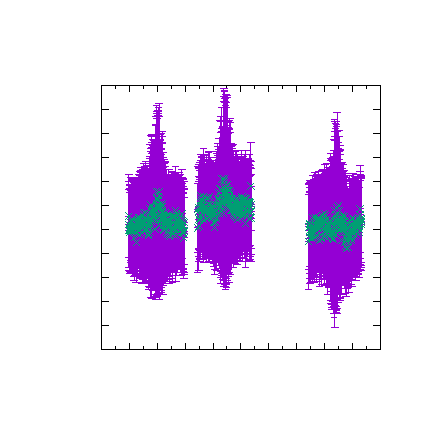
\includegraphics{../images/20160222_NO_fixI0_O3_ts}}%
    \gplfronttext
  \end{picture}%
\endgroup

    }
    \caption{\ch{NO2} and \ch{O3} time series at different set \ch{NO}
      flows and different reaction tube length.}
    \label{fig:flow}
  \end{figure}
\end{frame}

\begin{frame}
  \frametitle{Measurements}
  \framesubtitle{Pure \ch{NO} measurements in synthetic air}
  \begin{align*}
    y = \num{0.994\pm 0.002} \cdot x - \num{0.002 \pm 0.058}
  \end{align*}

  \begin{figure}[htbp]
    \centering
    \scalebox{.6}{
      % GNUPLOT: LaTeX picture with Postscript
\begingroup
  \makeatletter
  \providecommand\color[2][]{%
    \GenericError{(gnuplot) \space\space\space\@spaces}{%
      Package color not loaded in conjunction with
      terminal option `colourtext'%
    }{See the gnuplot documentation for explanation.%
    }{Either use 'blacktext' in gnuplot or load the package
      color.sty in LaTeX.}%
    \renewcommand\color[2][]{}%
  }%
  \providecommand\includegraphics[2][]{%
    \GenericError{(gnuplot) \space\space\space\@spaces}{%
      Package graphicx or graphics not loaded%
    }{See the gnuplot documentation for explanation.%
    }{The gnuplot epslatex terminal needs graphicx.sty or graphics.sty.}%
    \renewcommand\includegraphics[2][]{}%
  }%
  \providecommand\rotatebox[2]{#2}%
  \@ifundefined{ifGPcolor}{%
    \newif\ifGPcolor
    \GPcolorfalse
  }{}%
  \@ifundefined{ifGPblacktext}{%
    \newif\ifGPblacktext
    \GPblacktexttrue
  }{}%
  % define a \g@addto@macro without @ in the name:
  \let\gplgaddtomacro\g@addto@macro
  % define empty templates for all commands taking text:
  \gdef\gplbacktext{}%
  \gdef\gplfronttext{}%
  \makeatother
  \ifGPblacktext
    % no textcolor at all
    \def\colorrgb#1{}%
    \def\colorgray#1{}%
  \else
    % gray or color?
    \ifGPcolor
      \def\colorrgb#1{\color[rgb]{#1}}%
      \def\colorgray#1{\color[gray]{#1}}%
      \expandafter\def\csname LTw\endcsname{\color{white}}%
      \expandafter\def\csname LTb\endcsname{\color{black}}%
      \expandafter\def\csname LTa\endcsname{\color{black}}%
      \expandafter\def\csname LT0\endcsname{\color[rgb]{1,0,0}}%
      \expandafter\def\csname LT1\endcsname{\color[rgb]{0,1,0}}%
      \expandafter\def\csname LT2\endcsname{\color[rgb]{0,0,1}}%
      \expandafter\def\csname LT3\endcsname{\color[rgb]{1,0,1}}%
      \expandafter\def\csname LT4\endcsname{\color[rgb]{0,1,1}}%
      \expandafter\def\csname LT5\endcsname{\color[rgb]{1,1,0}}%
      \expandafter\def\csname LT6\endcsname{\color[rgb]{0,0,0}}%
      \expandafter\def\csname LT7\endcsname{\color[rgb]{1,0.3,0}}%
      \expandafter\def\csname LT8\endcsname{\color[rgb]{0.5,0.5,0.5}}%
    \else
      % gray
      \def\colorrgb#1{\color{black}}%
      \def\colorgray#1{\color[gray]{#1}}%
      \expandafter\def\csname LTw\endcsname{\color{white}}%
      \expandafter\def\csname LTb\endcsname{\color{black}}%
      \expandafter\def\csname LTa\endcsname{\color{black}}%
      \expandafter\def\csname LT0\endcsname{\color{black}}%
      \expandafter\def\csname LT1\endcsname{\color{black}}%
      \expandafter\def\csname LT2\endcsname{\color{black}}%
      \expandafter\def\csname LT3\endcsname{\color{black}}%
      \expandafter\def\csname LT4\endcsname{\color{black}}%
      \expandafter\def\csname LT5\endcsname{\color{black}}%
      \expandafter\def\csname LT6\endcsname{\color{black}}%
      \expandafter\def\csname LT7\endcsname{\color{black}}%
      \expandafter\def\csname LT8\endcsname{\color{black}}%
    \fi
  \fi
    \setlength{\unitlength}{0.0500bp}%
    \ifx\gptboxheight\undefined%
      \newlength{\gptboxheight}%
      \newlength{\gptboxwidth}%
      \newsavebox{\gptboxtext}%
    \fi%
    \setlength{\fboxrule}{0.5pt}%
    \setlength{\fboxsep}{1pt}%
\begin{picture}(7776.00,4320.00)%
    \gplgaddtomacro\gplbacktext{%
      \csname LTb\endcsname%
      \put(682,704){\makebox(0,0)[r]{\strut{}$0$}}%
      \put(682,1076){\makebox(0,0)[r]{\strut{}$10$}}%
      \put(682,1449){\makebox(0,0)[r]{\strut{}$20$}}%
      \put(682,1821){\makebox(0,0)[r]{\strut{}$30$}}%
      \put(682,2193){\makebox(0,0)[r]{\strut{}$40$}}%
      \put(682,2566){\makebox(0,0)[r]{\strut{}$50$}}%
      \put(682,2938){\makebox(0,0)[r]{\strut{}$60$}}%
      \put(682,3310){\makebox(0,0)[r]{\strut{}$70$}}%
      \put(682,3683){\makebox(0,0)[r]{\strut{}$80$}}%
      \put(682,4055){\makebox(0,0)[r]{\strut{}$90$}}%
      \put(814,484){\makebox(0,0){\strut{}$0$}}%
      \put(1543,484){\makebox(0,0){\strut{}$10$}}%
      \put(2273,484){\makebox(0,0){\strut{}$20$}}%
      \put(3002,484){\makebox(0,0){\strut{}$30$}}%
      \put(3732,484){\makebox(0,0){\strut{}$40$}}%
      \put(4461,484){\makebox(0,0){\strut{}$50$}}%
      \put(5191,484){\makebox(0,0){\strut{}$60$}}%
      \put(5920,484){\makebox(0,0){\strut{}$70$}}%
      \put(6650,484){\makebox(0,0){\strut{}$80$}}%
      \put(7379,484){\makebox(0,0){\strut{}$90$}}%
    }%
    \gplgaddtomacro\gplfronttext{%
      \csname LTb\endcsname%
      \put(176,2379){\rotatebox{-270}{\makebox(0,0){\strut{}\ch{NO} Concentration, measured with ICAD [ppb]}}}%
      \put(4096,154){\makebox(0,0){\strut{}\ch{NO} Concentration, calculated [ppb]}}%
    }%
    \gplbacktext
    \put(0,0){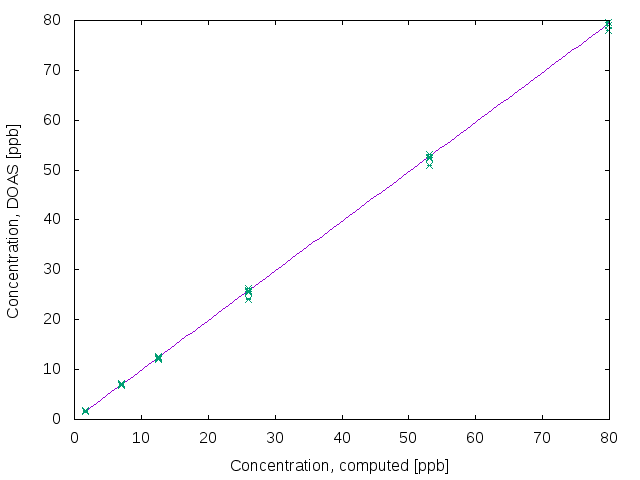
\includegraphics{../images/20160222_NO_fixI0}}%
    \gplfronttext
  \end{picture}%
\endgroup

    }
    \caption{Correlation plot between the measured and the calculated
      \ch{NO} concentration.}
    \label{fig:flow}
  \end{figure}
\end{frame}

\begin{frame}
  \frametitle{Measurements}
  \framesubtitle{Tuning behavior after Ozone switches}
  \begin{figure}[htbp]
    \centering
    \scalebox{.6}{
      % GNUPLOT: LaTeX picture with Postscript
\begingroup
  \makeatletter
  \providecommand\color[2][]{%
    \GenericError{(gnuplot) \space\space\space\@spaces}{%
      Package color not loaded in conjunction with
      terminal option `colourtext'%
    }{See the gnuplot documentation for explanation.%
    }{Either use 'blacktext' in gnuplot or load the package
      color.sty in LaTeX.}%
    \renewcommand\color[2][]{}%
  }%
  \providecommand\includegraphics[2][]{%
    \GenericError{(gnuplot) \space\space\space\@spaces}{%
      Package graphicx or graphics not loaded%
    }{See the gnuplot documentation for explanation.%
    }{The gnuplot epslatex terminal needs graphicx.sty or graphics.sty.}%
    \renewcommand\includegraphics[2][]{}%
  }%
  \providecommand\rotatebox[2]{#2}%
  \@ifundefined{ifGPcolor}{%
    \newif\ifGPcolor
    \GPcolorfalse
  }{}%
  \@ifundefined{ifGPblacktext}{%
    \newif\ifGPblacktext
    \GPblacktexttrue
  }{}%
  % define a \g@addto@macro without @ in the name:
  \let\gplgaddtomacro\g@addto@macro
  % define empty templates for all commands taking text:
  \gdef\gplbacktext{}%
  \gdef\gplfronttext{}%
  \makeatother
  \ifGPblacktext
    % no textcolor at all
    \def\colorrgb#1{}%
    \def\colorgray#1{}%
  \else
    % gray or color?
    \ifGPcolor
      \def\colorrgb#1{\color[rgb]{#1}}%
      \def\colorgray#1{\color[gray]{#1}}%
      \expandafter\def\csname LTw\endcsname{\color{white}}%
      \expandafter\def\csname LTb\endcsname{\color{black}}%
      \expandafter\def\csname LTa\endcsname{\color{black}}%
      \expandafter\def\csname LT0\endcsname{\color[rgb]{1,0,0}}%
      \expandafter\def\csname LT1\endcsname{\color[rgb]{0,1,0}}%
      \expandafter\def\csname LT2\endcsname{\color[rgb]{0,0,1}}%
      \expandafter\def\csname LT3\endcsname{\color[rgb]{1,0,1}}%
      \expandafter\def\csname LT4\endcsname{\color[rgb]{0,1,1}}%
      \expandafter\def\csname LT5\endcsname{\color[rgb]{1,1,0}}%
      \expandafter\def\csname LT6\endcsname{\color[rgb]{0,0,0}}%
      \expandafter\def\csname LT7\endcsname{\color[rgb]{1,0.3,0}}%
      \expandafter\def\csname LT8\endcsname{\color[rgb]{0.5,0.5,0.5}}%
    \else
      % gray
      \def\colorrgb#1{\color{black}}%
      \def\colorgray#1{\color[gray]{#1}}%
      \expandafter\def\csname LTw\endcsname{\color{white}}%
      \expandafter\def\csname LTb\endcsname{\color{black}}%
      \expandafter\def\csname LTa\endcsname{\color{black}}%
      \expandafter\def\csname LT0\endcsname{\color{black}}%
      \expandafter\def\csname LT1\endcsname{\color{black}}%
      \expandafter\def\csname LT2\endcsname{\color{black}}%
      \expandafter\def\csname LT3\endcsname{\color{black}}%
      \expandafter\def\csname LT4\endcsname{\color{black}}%
      \expandafter\def\csname LT5\endcsname{\color{black}}%
      \expandafter\def\csname LT6\endcsname{\color{black}}%
      \expandafter\def\csname LT7\endcsname{\color{black}}%
      \expandafter\def\csname LT8\endcsname{\color{black}}%
    \fi
  \fi
    \setlength{\unitlength}{0.0500bp}%
    \ifx\gptboxheight\undefined%
      \newlength{\gptboxheight}%
      \newlength{\gptboxwidth}%
      \newsavebox{\gptboxtext}%
    \fi%
    \setlength{\fboxrule}{0.5pt}%
    \setlength{\fboxsep}{1pt}%
\begin{picture}(7200.00,5040.00)%
    \gplgaddtomacro\gplbacktext{%
      \csname LTb\endcsname%
      \put(682,704){\makebox(0,0)[r]{\strut{}$0$}}%
      \put(682,1383){\makebox(0,0)[r]{\strut{}$5$}}%
      \put(682,2061){\makebox(0,0)[r]{\strut{}$10$}}%
      \put(682,2740){\makebox(0,0)[r]{\strut{}$15$}}%
      \put(682,3418){\makebox(0,0)[r]{\strut{}$20$}}%
      \put(682,4097){\makebox(0,0)[r]{\strut{}$25$}}%
      \put(682,4775){\makebox(0,0)[r]{\strut{}$30$}}%
      \put(814,484){\makebox(0,0){\strut{}$0$}}%
      \put(1563,484){\makebox(0,0){\strut{}$500$}}%
      \put(2311,484){\makebox(0,0){\strut{}$1000$}}%
      \put(3060,484){\makebox(0,0){\strut{}$1500$}}%
      \put(3809,484){\makebox(0,0){\strut{}$2000$}}%
      \put(4557,484){\makebox(0,0){\strut{}$2500$}}%
      \put(5306,484){\makebox(0,0){\strut{}$3000$}}%
      \put(6054,484){\makebox(0,0){\strut{}$3500$}}%
      \put(6803,484){\makebox(0,0){\strut{}$4000$}}%
    }%
    \gplgaddtomacro\gplfronttext{%
      \csname LTb\endcsname%
      \put(176,2739){\rotatebox{-270}{\makebox(0,0){\strut{}Concentration [ppb]}}}%
      \put(3808,154){\makebox(0,0){\strut{}Time [s]}}%
    }%
    \gplbacktext
    \put(0,0){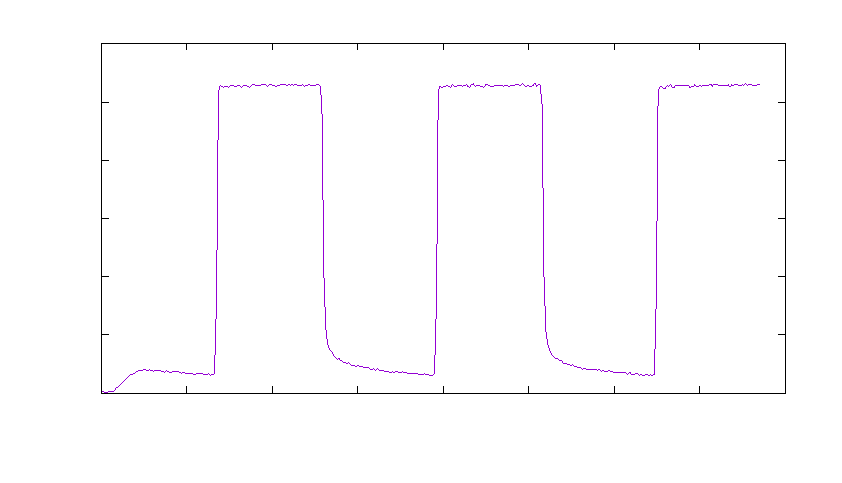
\includegraphics{../images/20160223_15_equil_fixI0_ts}}%
    \gplfronttext
  \end{picture}%
\endgroup

    }
    \caption{Time series of the \ch{NO2} concentration at a fixed
      \ch{NO} flow while turning the \ch{O3} on and off. Reaction tube
    length \(l= \SI{15}{\meter}\).}
    \label{fig:flow}
  \end{figure}
\end{frame}

\begin{frame}
  \frametitle{Measurements}
  \framesubtitle{Tuning behavior after Ozone switches}
  \begin{figure}[htbp]
    \centering
    \scalebox{.6}{
      % GNUPLOT: LaTeX picture with Postscript
\begingroup
  \makeatletter
  \providecommand\color[2][]{%
    \GenericError{(gnuplot) \space\space\space\@spaces}{%
      Package color not loaded in conjunction with
      terminal option `colourtext'%
    }{See the gnuplot documentation for explanation.%
    }{Either use 'blacktext' in gnuplot or load the package
      color.sty in LaTeX.}%
    \renewcommand\color[2][]{}%
  }%
  \providecommand\includegraphics[2][]{%
    \GenericError{(gnuplot) \space\space\space\@spaces}{%
      Package graphicx or graphics not loaded%
    }{See the gnuplot documentation for explanation.%
    }{The gnuplot epslatex terminal needs graphicx.sty or graphics.sty.}%
    \renewcommand\includegraphics[2][]{}%
  }%
  \providecommand\rotatebox[2]{#2}%
  \@ifundefined{ifGPcolor}{%
    \newif\ifGPcolor
    \GPcolorfalse
  }{}%
  \@ifundefined{ifGPblacktext}{%
    \newif\ifGPblacktext
    \GPblacktexttrue
  }{}%
  % define a \g@addto@macro without @ in the name:
  \let\gplgaddtomacro\g@addto@macro
  % define empty templates for all commands taking text:
  \gdef\gplbacktext{}%
  \gdef\gplfronttext{}%
  \makeatother
  \ifGPblacktext
    % no textcolor at all
    \def\colorrgb#1{}%
    \def\colorgray#1{}%
  \else
    % gray or color?
    \ifGPcolor
      \def\colorrgb#1{\color[rgb]{#1}}%
      \def\colorgray#1{\color[gray]{#1}}%
      \expandafter\def\csname LTw\endcsname{\color{white}}%
      \expandafter\def\csname LTb\endcsname{\color{black}}%
      \expandafter\def\csname LTa\endcsname{\color{black}}%
      \expandafter\def\csname LT0\endcsname{\color[rgb]{1,0,0}}%
      \expandafter\def\csname LT1\endcsname{\color[rgb]{0,1,0}}%
      \expandafter\def\csname LT2\endcsname{\color[rgb]{0,0,1}}%
      \expandafter\def\csname LT3\endcsname{\color[rgb]{1,0,1}}%
      \expandafter\def\csname LT4\endcsname{\color[rgb]{0,1,1}}%
      \expandafter\def\csname LT5\endcsname{\color[rgb]{1,1,0}}%
      \expandafter\def\csname LT6\endcsname{\color[rgb]{0,0,0}}%
      \expandafter\def\csname LT7\endcsname{\color[rgb]{1,0.3,0}}%
      \expandafter\def\csname LT8\endcsname{\color[rgb]{0.5,0.5,0.5}}%
    \else
      % gray
      \def\colorrgb#1{\color{black}}%
      \def\colorgray#1{\color[gray]{#1}}%
      \expandafter\def\csname LTw\endcsname{\color{white}}%
      \expandafter\def\csname LTb\endcsname{\color{black}}%
      \expandafter\def\csname LTa\endcsname{\color{black}}%
      \expandafter\def\csname LT0\endcsname{\color{black}}%
      \expandafter\def\csname LT1\endcsname{\color{black}}%
      \expandafter\def\csname LT2\endcsname{\color{black}}%
      \expandafter\def\csname LT3\endcsname{\color{black}}%
      \expandafter\def\csname LT4\endcsname{\color{black}}%
      \expandafter\def\csname LT5\endcsname{\color{black}}%
      \expandafter\def\csname LT6\endcsname{\color{black}}%
      \expandafter\def\csname LT7\endcsname{\color{black}}%
      \expandafter\def\csname LT8\endcsname{\color{black}}%
    \fi
  \fi
    \setlength{\unitlength}{0.0500bp}%
    \ifx\gptboxheight\undefined%
      \newlength{\gptboxheight}%
      \newlength{\gptboxwidth}%
      \newsavebox{\gptboxtext}%
    \fi%
    \setlength{\fboxrule}{0.5pt}%
    \setlength{\fboxsep}{1pt}%
\begin{picture}(7200.00,5040.00)%
    \gplgaddtomacro\gplbacktext{%
      \csname LTb\endcsname%
      \put(682,704){\makebox(0,0)[r]{\strut{}$0$}}%
      \put(682,1518){\makebox(0,0)[r]{\strut{}$5$}}%
      \put(682,2332){\makebox(0,0)[r]{\strut{}$10$}}%
      \put(682,3147){\makebox(0,0)[r]{\strut{}$15$}}%
      \put(682,3961){\makebox(0,0)[r]{\strut{}$20$}}%
      \put(682,4775){\makebox(0,0)[r]{\strut{}$25$}}%
      \put(814,484){\makebox(0,0){\strut{}$0$}}%
      \put(1670,484){\makebox(0,0){\strut{}$100$}}%
      \put(2525,484){\makebox(0,0){\strut{}$200$}}%
      \put(3381,484){\makebox(0,0){\strut{}$300$}}%
      \put(4236,484){\makebox(0,0){\strut{}$400$}}%
      \put(5092,484){\makebox(0,0){\strut{}$500$}}%
      \put(5947,484){\makebox(0,0){\strut{}$600$}}%
      \put(6803,484){\makebox(0,0){\strut{}$700$}}%
    }%
    \gplgaddtomacro\gplfronttext{%
      \csname LTb\endcsname%
      \put(176,2739){\rotatebox{-270}{\makebox(0,0){\strut{}Concentration [ppb]}}}%
      \put(3808,154){\makebox(0,0){\strut{}Time [s]}}%
      \csname LTb\endcsname%
      \put(5816,4602){\makebox(0,0)[r]{\strut{}$\SI{05}{\meter}$}}%
      \csname LTb\endcsname%
      \put(5816,4382){\makebox(0,0)[r]{\strut{}$\SI{10}{\meter}$}}%
      \csname LTb\endcsname%
      \put(5816,4162){\makebox(0,0)[r]{\strut{}$\SI{15}{\meter}$}}%
    }%
    \gplbacktext
    \put(0,0){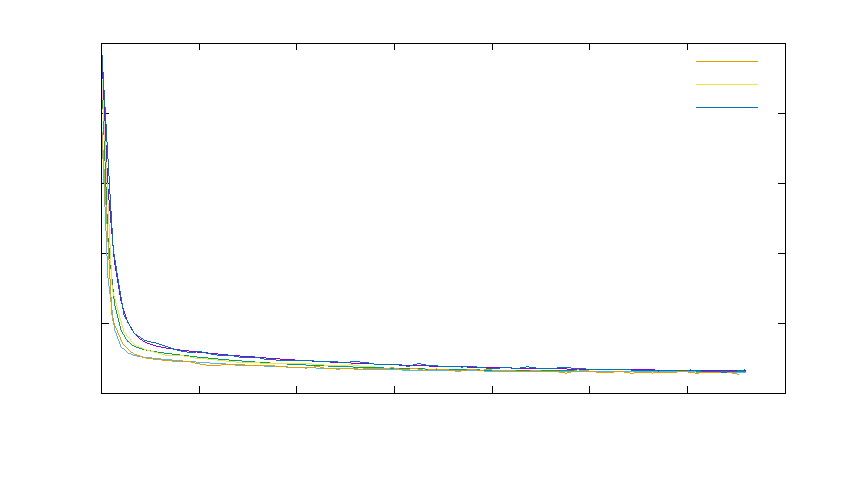
\includegraphics{../images/20160223_equil_fixI0_fall_fit}}%
    \gplfronttext
  \end{picture}%
\endgroup

    }
    \caption{Time series of the \ch{NO2} concentration after the
      \ch{O3} had been turned off.}
    \label{fig:flow}
  \end{figure}
\end{frame}

\begin{frame}
  \frametitle{Measurements}
  \framesubtitle{Comparison of the alternating measurement mode to a
    chemiluminescence display}
    \begin{figure}[htbp]
    \centering
    \scalebox{.7}{
      % GNUPLOT: LaTeX picture with Postscript
\begingroup
  \makeatletter
  \providecommand\color[2][]{%
    \GenericError{(gnuplot) \space\space\space\@spaces}{%
      Package color not loaded in conjunction with
      terminal option `colourtext'%
    }{See the gnuplot documentation for explanation.%
    }{Either use 'blacktext' in gnuplot or load the package
      color.sty in LaTeX.}%
    \renewcommand\color[2][]{}%
  }%
  \providecommand\includegraphics[2][]{%
    \GenericError{(gnuplot) \space\space\space\@spaces}{%
      Package graphicx or graphics not loaded%
    }{See the gnuplot documentation for explanation.%
    }{The gnuplot epslatex terminal needs graphicx.sty or graphics.sty.}%
    \renewcommand\includegraphics[2][]{}%
  }%
  \providecommand\rotatebox[2]{#2}%
  \@ifundefined{ifGPcolor}{%
    \newif\ifGPcolor
    \GPcolorfalse
  }{}%
  \@ifundefined{ifGPblacktext}{%
    \newif\ifGPblacktext
    \GPblacktexttrue
  }{}%
  % define a \g@addto@macro without @ in the name:
  \let\gplgaddtomacro\g@addto@macro
  % define empty templates for all commands taking text:
  \gdef\gplbacktext{}%
  \gdef\gplfronttext{}%
  \makeatother
  \ifGPblacktext
    % no textcolor at all
    \def\colorrgb#1{}%
    \def\colorgray#1{}%
  \else
    % gray or color?
    \ifGPcolor
      \def\colorrgb#1{\color[rgb]{#1}}%
      \def\colorgray#1{\color[gray]{#1}}%
      \expandafter\def\csname LTw\endcsname{\color{white}}%
      \expandafter\def\csname LTb\endcsname{\color{black}}%
      \expandafter\def\csname LTa\endcsname{\color{black}}%
      \expandafter\def\csname LT0\endcsname{\color[rgb]{1,0,0}}%
      \expandafter\def\csname LT1\endcsname{\color[rgb]{0,1,0}}%
      \expandafter\def\csname LT2\endcsname{\color[rgb]{0,0,1}}%
      \expandafter\def\csname LT3\endcsname{\color[rgb]{1,0,1}}%
      \expandafter\def\csname LT4\endcsname{\color[rgb]{0,1,1}}%
      \expandafter\def\csname LT5\endcsname{\color[rgb]{1,1,0}}%
      \expandafter\def\csname LT6\endcsname{\color[rgb]{0,0,0}}%
      \expandafter\def\csname LT7\endcsname{\color[rgb]{1,0.3,0}}%
      \expandafter\def\csname LT8\endcsname{\color[rgb]{0.5,0.5,0.5}}%
    \else
      % gray
      \def\colorrgb#1{\color{black}}%
      \def\colorgray#1{\color[gray]{#1}}%
      \expandafter\def\csname LTw\endcsname{\color{white}}%
      \expandafter\def\csname LTb\endcsname{\color{black}}%
      \expandafter\def\csname LTa\endcsname{\color{black}}%
      \expandafter\def\csname LT0\endcsname{\color{black}}%
      \expandafter\def\csname LT1\endcsname{\color{black}}%
      \expandafter\def\csname LT2\endcsname{\color{black}}%
      \expandafter\def\csname LT3\endcsname{\color{black}}%
      \expandafter\def\csname LT4\endcsname{\color{black}}%
      \expandafter\def\csname LT5\endcsname{\color{black}}%
      \expandafter\def\csname LT6\endcsname{\color{black}}%
      \expandafter\def\csname LT7\endcsname{\color{black}}%
      \expandafter\def\csname LT8\endcsname{\color{black}}%
    \fi
  \fi
    \setlength{\unitlength}{0.0500bp}%
    \ifx\gptboxheight\undefined%
      \newlength{\gptboxheight}%
      \newlength{\gptboxwidth}%
      \newsavebox{\gptboxtext}%
    \fi%
    \setlength{\fboxrule}{0.5pt}%
    \setlength{\fboxsep}{1pt}%
\begin{picture}(3888.00,3888.00)%
    \gplgaddtomacro\gplbacktext{%
      \csname LTb\endcsname%
      \put(682,686){\makebox(0,0)[r]{\strut{}$-5$}}%
      \put(682,917){\makebox(0,0)[r]{\strut{}$0$}}%
      \put(682,1148){\makebox(0,0)[r]{\strut{}$5$}}%
      \put(682,1379){\makebox(0,0)[r]{\strut{}$10$}}%
      \put(682,1610){\makebox(0,0)[r]{\strut{}$15$}}%
      \put(682,1841){\makebox(0,0)[r]{\strut{}$20$}}%
      \put(682,2072){\makebox(0,0)[r]{\strut{}$25$}}%
      \put(682,2303){\makebox(0,0)[r]{\strut{}$30$}}%
      \put(682,2534){\makebox(0,0)[r]{\strut{}$35$}}%
      \put(682,2765){\makebox(0,0)[r]{\strut{}$40$}}%
      \put(682,2996){\makebox(0,0)[r]{\strut{}$45$}}%
      \put(682,3227){\makebox(0,0)[r]{\strut{}$50$}}%
      \put(814,554){\rotatebox{-45}{\makebox(0,0)[l]{\strut{}16:00}}}%
      \put(1149,554){\rotatebox{-45}{\makebox(0,0)[l]{\strut{}17:00}}}%
      \put(1483,554){\rotatebox{-45}{\makebox(0,0)[l]{\strut{}18:00}}}%
      \put(1818,554){\rotatebox{-45}{\makebox(0,0)[l]{\strut{}19:00}}}%
      \put(2153,554){\rotatebox{-45}{\makebox(0,0)[l]{\strut{}20:00}}}%
      \put(2487,554){\rotatebox{-45}{\makebox(0,0)[l]{\strut{}21:00}}}%
      \put(2822,554){\rotatebox{-45}{\makebox(0,0)[l]{\strut{}22:00}}}%
      \put(3156,554){\rotatebox{-45}{\makebox(0,0)[l]{\strut{}23:00}}}%
      \put(3491,554){\rotatebox{-45}{\makebox(0,0)[l]{\strut{}00:00}}}%
    }%
    \gplgaddtomacro\gplfronttext{%
      \csname LTb\endcsname%
      \put(176,1956){\rotatebox{-270}{\makebox(0,0){\strut{}\ch{NO} Concentration [ppb]}}}%
      \put(2152,3557){\makebox(0,0){\strut{}January 22, 2016}}%
    }%
    \gplbacktext
    \put(0,0){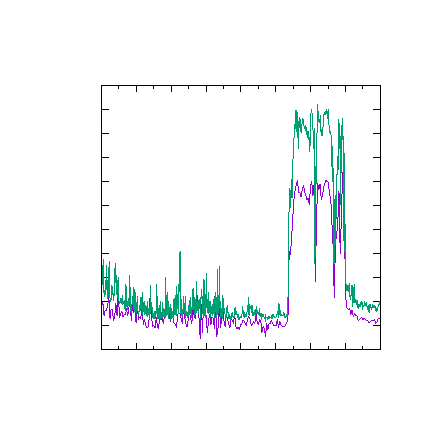
\includegraphics{../images/correlation_ts01}}%
    \gplfronttext
  \end{picture}%
\endgroup

    }
    \hspace{1cm}
    \scalebox{.7}{
      % GNUPLOT: LaTeX picture with Postscript
\begingroup
  \makeatletter
  \providecommand\color[2][]{%
    \GenericError{(gnuplot) \space\space\space\@spaces}{%
      Package color not loaded in conjunction with
      terminal option `colourtext'%
    }{See the gnuplot documentation for explanation.%
    }{Either use 'blacktext' in gnuplot or load the package
      color.sty in LaTeX.}%
    \renewcommand\color[2][]{}%
  }%
  \providecommand\includegraphics[2][]{%
    \GenericError{(gnuplot) \space\space\space\@spaces}{%
      Package graphicx or graphics not loaded%
    }{See the gnuplot documentation for explanation.%
    }{The gnuplot epslatex terminal needs graphicx.sty or graphics.sty.}%
    \renewcommand\includegraphics[2][]{}%
  }%
  \providecommand\rotatebox[2]{#2}%
  \@ifundefined{ifGPcolor}{%
    \newif\ifGPcolor
    \GPcolorfalse
  }{}%
  \@ifundefined{ifGPblacktext}{%
    \newif\ifGPblacktext
    \GPblacktexttrue
  }{}%
  % define a \g@addto@macro without @ in the name:
  \let\gplgaddtomacro\g@addto@macro
  % define empty templates for all commands taking text:
  \gdef\gplbacktext{}%
  \gdef\gplfronttext{}%
  \makeatother
  \ifGPblacktext
    % no textcolor at all
    \def\colorrgb#1{}%
    \def\colorgray#1{}%
  \else
    % gray or color?
    \ifGPcolor
      \def\colorrgb#1{\color[rgb]{#1}}%
      \def\colorgray#1{\color[gray]{#1}}%
      \expandafter\def\csname LTw\endcsname{\color{white}}%
      \expandafter\def\csname LTb\endcsname{\color{black}}%
      \expandafter\def\csname LTa\endcsname{\color{black}}%
      \expandafter\def\csname LT0\endcsname{\color[rgb]{1,0,0}}%
      \expandafter\def\csname LT1\endcsname{\color[rgb]{0,1,0}}%
      \expandafter\def\csname LT2\endcsname{\color[rgb]{0,0,1}}%
      \expandafter\def\csname LT3\endcsname{\color[rgb]{1,0,1}}%
      \expandafter\def\csname LT4\endcsname{\color[rgb]{0,1,1}}%
      \expandafter\def\csname LT5\endcsname{\color[rgb]{1,1,0}}%
      \expandafter\def\csname LT6\endcsname{\color[rgb]{0,0,0}}%
      \expandafter\def\csname LT7\endcsname{\color[rgb]{1,0.3,0}}%
      \expandafter\def\csname LT8\endcsname{\color[rgb]{0.5,0.5,0.5}}%
    \else
      % gray
      \def\colorrgb#1{\color{black}}%
      \def\colorgray#1{\color[gray]{#1}}%
      \expandafter\def\csname LTw\endcsname{\color{white}}%
      \expandafter\def\csname LTb\endcsname{\color{black}}%
      \expandafter\def\csname LTa\endcsname{\color{black}}%
      \expandafter\def\csname LT0\endcsname{\color{black}}%
      \expandafter\def\csname LT1\endcsname{\color{black}}%
      \expandafter\def\csname LT2\endcsname{\color{black}}%
      \expandafter\def\csname LT3\endcsname{\color{black}}%
      \expandafter\def\csname LT4\endcsname{\color{black}}%
      \expandafter\def\csname LT5\endcsname{\color{black}}%
      \expandafter\def\csname LT6\endcsname{\color{black}}%
      \expandafter\def\csname LT7\endcsname{\color{black}}%
      \expandafter\def\csname LT8\endcsname{\color{black}}%
    \fi
  \fi
    \setlength{\unitlength}{0.0500bp}%
    \ifx\gptboxheight\undefined%
      \newlength{\gptboxheight}%
      \newlength{\gptboxwidth}%
      \newsavebox{\gptboxtext}%
    \fi%
    \setlength{\fboxrule}{0.5pt}%
    \setlength{\fboxsep}{1pt}%
\begin{picture}(3888.00,3888.00)%
    \gplgaddtomacro\gplbacktext{%
      \csname LTb\endcsname%
      \put(814,686){\makebox(0,0)[r]{\strut{}$-10$}}%
      \put(814,1049){\makebox(0,0)[r]{\strut{}$0$}}%
      \put(814,1412){\makebox(0,0)[r]{\strut{}$10$}}%
      \put(814,1775){\makebox(0,0)[r]{\strut{}$20$}}%
      \put(814,2138){\makebox(0,0)[r]{\strut{}$30$}}%
      \put(814,2501){\makebox(0,0)[r]{\strut{}$40$}}%
      \put(814,2864){\makebox(0,0)[r]{\strut{}$50$}}%
      \put(814,3227){\makebox(0,0)[r]{\strut{}$60$}}%
      \put(946,554){\rotatebox{-45}{\makebox(0,0)[l]{\strut{}08:00}}}%
      \put(1264,554){\rotatebox{-45}{\makebox(0,0)[l]{\strut{}10:00}}}%
      \put(1582,554){\rotatebox{-45}{\makebox(0,0)[l]{\strut{}12:00}}}%
      \put(1900,554){\rotatebox{-45}{\makebox(0,0)[l]{\strut{}14:00}}}%
      \put(2219,554){\rotatebox{-45}{\makebox(0,0)[l]{\strut{}16:00}}}%
      \put(2537,554){\rotatebox{-45}{\makebox(0,0)[l]{\strut{}18:00}}}%
      \put(2855,554){\rotatebox{-45}{\makebox(0,0)[l]{\strut{}20:00}}}%
      \put(3173,554){\rotatebox{-45}{\makebox(0,0)[l]{\strut{}22:00}}}%
      \put(3491,554){\rotatebox{-45}{\makebox(0,0)[l]{\strut{}00:00}}}%
    }%
    \gplgaddtomacro\gplfronttext{%
      \csname LTb\endcsname%
      \put(176,1956){\rotatebox{-270}{\makebox(0,0){\strut{}Concentration [ppb]}}}%
      \put(2218,3557){\makebox(0,0){\strut{}January 25, 2016}}%
      \csname LTb\endcsname%
      \put(2504,3054){\makebox(0,0)[r]{\strut{}DOAS}}%
      \csname LTb\endcsname%
      \put(2504,2834){\makebox(0,0)[r]{\strut{}CLD}}%
    }%
    \gplbacktext
    \put(0,0){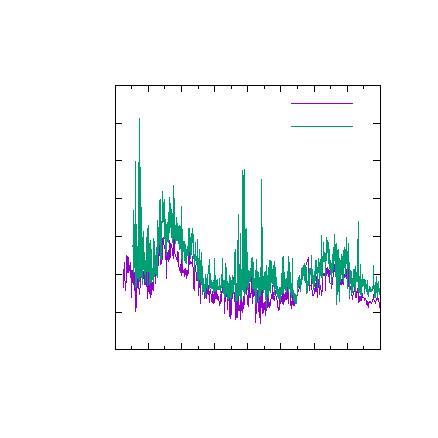
\includegraphics{../images/correlation_ts02}}%
    \gplfronttext
  \end{picture}%
\endgroup

    }
    \caption{\ch{NO} time series as determined by the ICAD instrument
      and the chemiluminescence display.}
    \label{fig:flow}
  \end{figure}
\end{frame}

\begin{frame}
  \frametitle{Measurements}
  \framesubtitle{Comparison of the alternating measurement mode to a
    chemiluminescence display}
  \begin{align*}
    y & = 1.38\text{ ppb}^{-1} \cdot x + 3.8 && \text{uncorrected}\\
    y & = 1.38\text{ ppb}^{-1} \cdot x + 1.67 && \text{`naively' tail corrected} 
  \end{align*}
  \begin{figure}[htbp]
    \centering
    \scalebox{.55}{
      % GNUPLOT: LaTeX picture with Postscript
\begingroup
  \makeatletter
  \providecommand\color[2][]{%
    \GenericError{(gnuplot) \space\space\space\@spaces}{%
      Package color not loaded in conjunction with
      terminal option `colourtext'%
    }{See the gnuplot documentation for explanation.%
    }{Either use 'blacktext' in gnuplot or load the package
      color.sty in LaTeX.}%
    \renewcommand\color[2][]{}%
  }%
  \providecommand\includegraphics[2][]{%
    \GenericError{(gnuplot) \space\space\space\@spaces}{%
      Package graphicx or graphics not loaded%
    }{See the gnuplot documentation for explanation.%
    }{The gnuplot epslatex terminal needs graphicx.sty or graphics.sty.}%
    \renewcommand\includegraphics[2][]{}%
  }%
  \providecommand\rotatebox[2]{#2}%
  \@ifundefined{ifGPcolor}{%
    \newif\ifGPcolor
    \GPcolorfalse
  }{}%
  \@ifundefined{ifGPblacktext}{%
    \newif\ifGPblacktext
    \GPblacktexttrue
  }{}%
  % define a \g@addto@macro without @ in the name:
  \let\gplgaddtomacro\g@addto@macro
  % define empty templates for all commands taking text:
  \gdef\gplbacktext{}%
  \gdef\gplfronttext{}%
  \makeatother
  \ifGPblacktext
    % no textcolor at all
    \def\colorrgb#1{}%
    \def\colorgray#1{}%
  \else
    % gray or color?
    \ifGPcolor
      \def\colorrgb#1{\color[rgb]{#1}}%
      \def\colorgray#1{\color[gray]{#1}}%
      \expandafter\def\csname LTw\endcsname{\color{white}}%
      \expandafter\def\csname LTb\endcsname{\color{black}}%
      \expandafter\def\csname LTa\endcsname{\color{black}}%
      \expandafter\def\csname LT0\endcsname{\color[rgb]{1,0,0}}%
      \expandafter\def\csname LT1\endcsname{\color[rgb]{0,1,0}}%
      \expandafter\def\csname LT2\endcsname{\color[rgb]{0,0,1}}%
      \expandafter\def\csname LT3\endcsname{\color[rgb]{1,0,1}}%
      \expandafter\def\csname LT4\endcsname{\color[rgb]{0,1,1}}%
      \expandafter\def\csname LT5\endcsname{\color[rgb]{1,1,0}}%
      \expandafter\def\csname LT6\endcsname{\color[rgb]{0,0,0}}%
      \expandafter\def\csname LT7\endcsname{\color[rgb]{1,0.3,0}}%
      \expandafter\def\csname LT8\endcsname{\color[rgb]{0.5,0.5,0.5}}%
    \else
      % gray
      \def\colorrgb#1{\color{black}}%
      \def\colorgray#1{\color[gray]{#1}}%
      \expandafter\def\csname LTw\endcsname{\color{white}}%
      \expandafter\def\csname LTb\endcsname{\color{black}}%
      \expandafter\def\csname LTa\endcsname{\color{black}}%
      \expandafter\def\csname LT0\endcsname{\color{black}}%
      \expandafter\def\csname LT1\endcsname{\color{black}}%
      \expandafter\def\csname LT2\endcsname{\color{black}}%
      \expandafter\def\csname LT3\endcsname{\color{black}}%
      \expandafter\def\csname LT4\endcsname{\color{black}}%
      \expandafter\def\csname LT5\endcsname{\color{black}}%
      \expandafter\def\csname LT6\endcsname{\color{black}}%
      \expandafter\def\csname LT7\endcsname{\color{black}}%
      \expandafter\def\csname LT8\endcsname{\color{black}}%
    \fi
  \fi
    \setlength{\unitlength}{0.0500bp}%
    \ifx\gptboxheight\undefined%
      \newlength{\gptboxheight}%
      \newlength{\gptboxwidth}%
      \newsavebox{\gptboxtext}%
    \fi%
    \setlength{\fboxrule}{0.5pt}%
    \setlength{\fboxsep}{1pt}%
\begin{picture}(7776.00,4320.00)%
    \gplgaddtomacro\gplbacktext{%
      \csname LTb\endcsname%
      \put(682,704){\makebox(0,0)[r]{\strut{}$-5$}}%
      \put(682,1039){\makebox(0,0)[r]{\strut{}$0$}}%
      \put(682,1374){\makebox(0,0)[r]{\strut{}$5$}}%
      \put(682,1709){\makebox(0,0)[r]{\strut{}$10$}}%
      \put(682,2044){\makebox(0,0)[r]{\strut{}$15$}}%
      \put(682,2380){\makebox(0,0)[r]{\strut{}$20$}}%
      \put(682,2715){\makebox(0,0)[r]{\strut{}$25$}}%
      \put(682,3050){\makebox(0,0)[r]{\strut{}$30$}}%
      \put(682,3385){\makebox(0,0)[r]{\strut{}$35$}}%
      \put(682,3720){\makebox(0,0)[r]{\strut{}$40$}}%
      \put(682,4055){\makebox(0,0)[r]{\strut{}$45$}}%
      \put(814,484){\makebox(0,0){\strut{}$-5$}}%
      \put(1752,484){\makebox(0,0){\strut{}$0$}}%
      \put(2690,484){\makebox(0,0){\strut{}$5$}}%
      \put(3628,484){\makebox(0,0){\strut{}$10$}}%
      \put(4565,484){\makebox(0,0){\strut{}$15$}}%
      \put(5503,484){\makebox(0,0){\strut{}$20$}}%
      \put(6441,484){\makebox(0,0){\strut{}$25$}}%
      \put(7379,484){\makebox(0,0){\strut{}$30$}}%
    }%
    \gplgaddtomacro\gplfronttext{%
      \csname LTb\endcsname%
      \put(176,2379){\rotatebox{-270}{\makebox(0,0){\strut{}Concentration (CLD) [ppb]}}}%
      \put(4096,154){\makebox(0,0){\strut{}Concentration (ICAD) [ppb]}}%
      \csname LTb\endcsname%
      \put(3322,3882){\makebox(0,0)[r]{\strut{}uncorrected}}%
      \csname LTb\endcsname%
      \put(3322,3662){\makebox(0,0)[r]{\strut{}fit uncorrected}}%
      \csname LTb\endcsname%
      \put(3322,3442){\makebox(0,0)[r]{\strut{}tail corrected}}%
      \csname LTb\endcsname%
      \put(3322,3222){\makebox(0,0)[r]{\strut{}fit tail corrected}}%
    }%
    \gplbacktext
    \put(0,0){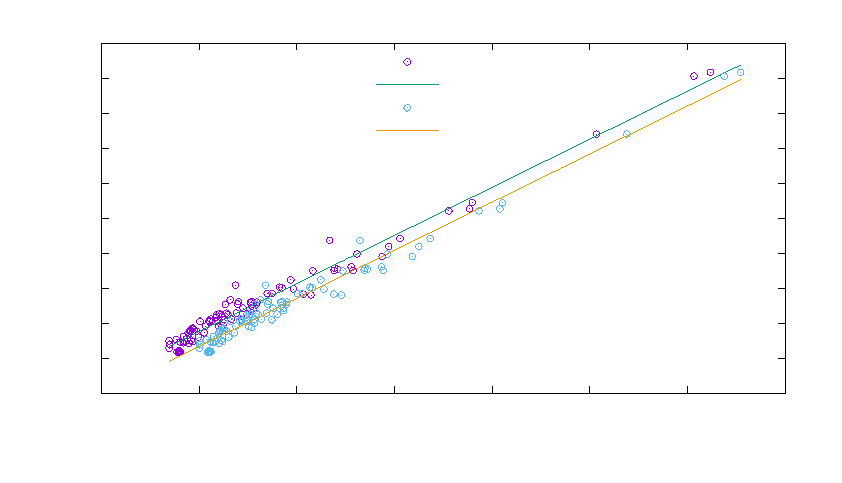
\includegraphics{../images/Correlation_corrected}}%
    \gplfronttext
  \end{picture}%
\endgroup

    }
    \caption{Correlation between the ICAD instrument and the
      CLD.}
    \label{fig:flow}
  \end{figure}
\end{frame}

% \begin{frame}
%   \frametitle{Measurements}
%   \begin{align*}
%     y & = \num{0.99 \pm 0.01} \cdot x + \num{0.6\pm0.3}\\
%   \end{align*}
%   \begin{figure}[htbp]
%     \centering
%     \scalebox{.6}{
%       % GNUPLOT: LaTeX picture with Postscript
\begingroup
  \makeatletter
  \providecommand\color[2][]{%
    \GenericError{(gnuplot) \space\space\space\@spaces}{%
      Package color not loaded in conjunction with
      terminal option `colourtext'%
    }{See the gnuplot documentation for explanation.%
    }{Either use 'blacktext' in gnuplot or load the package
      color.sty in LaTeX.}%
    \renewcommand\color[2][]{}%
  }%
  \providecommand\includegraphics[2][]{%
    \GenericError{(gnuplot) \space\space\space\@spaces}{%
      Package graphicx or graphics not loaded%
    }{See the gnuplot documentation for explanation.%
    }{The gnuplot epslatex terminal needs graphicx.sty or graphics.sty.}%
    \renewcommand\includegraphics[2][]{}%
  }%
  \providecommand\rotatebox[2]{#2}%
  \@ifundefined{ifGPcolor}{%
    \newif\ifGPcolor
    \GPcolorfalse
  }{}%
  \@ifundefined{ifGPblacktext}{%
    \newif\ifGPblacktext
    \GPblacktexttrue
  }{}%
  % define a \g@addto@macro without @ in the name:
  \let\gplgaddtomacro\g@addto@macro
  % define empty templates for all commands taking text:
  \gdef\gplbacktext{}%
  \gdef\gplfronttext{}%
  \makeatother
  \ifGPblacktext
    % no textcolor at all
    \def\colorrgb#1{}%
    \def\colorgray#1{}%
  \else
    % gray or color?
    \ifGPcolor
      \def\colorrgb#1{\color[rgb]{#1}}%
      \def\colorgray#1{\color[gray]{#1}}%
      \expandafter\def\csname LTw\endcsname{\color{white}}%
      \expandafter\def\csname LTb\endcsname{\color{black}}%
      \expandafter\def\csname LTa\endcsname{\color{black}}%
      \expandafter\def\csname LT0\endcsname{\color[rgb]{1,0,0}}%
      \expandafter\def\csname LT1\endcsname{\color[rgb]{0,1,0}}%
      \expandafter\def\csname LT2\endcsname{\color[rgb]{0,0,1}}%
      \expandafter\def\csname LT3\endcsname{\color[rgb]{1,0,1}}%
      \expandafter\def\csname LT4\endcsname{\color[rgb]{0,1,1}}%
      \expandafter\def\csname LT5\endcsname{\color[rgb]{1,1,0}}%
      \expandafter\def\csname LT6\endcsname{\color[rgb]{0,0,0}}%
      \expandafter\def\csname LT7\endcsname{\color[rgb]{1,0.3,0}}%
      \expandafter\def\csname LT8\endcsname{\color[rgb]{0.5,0.5,0.5}}%
    \else
      % gray
      \def\colorrgb#1{\color{black}}%
      \def\colorgray#1{\color[gray]{#1}}%
      \expandafter\def\csname LTw\endcsname{\color{white}}%
      \expandafter\def\csname LTb\endcsname{\color{black}}%
      \expandafter\def\csname LTa\endcsname{\color{black}}%
      \expandafter\def\csname LT0\endcsname{\color{black}}%
      \expandafter\def\csname LT1\endcsname{\color{black}}%
      \expandafter\def\csname LT2\endcsname{\color{black}}%
      \expandafter\def\csname LT3\endcsname{\color{black}}%
      \expandafter\def\csname LT4\endcsname{\color{black}}%
      \expandafter\def\csname LT5\endcsname{\color{black}}%
      \expandafter\def\csname LT6\endcsname{\color{black}}%
      \expandafter\def\csname LT7\endcsname{\color{black}}%
      \expandafter\def\csname LT8\endcsname{\color{black}}%
    \fi
  \fi
    \setlength{\unitlength}{0.0500bp}%
    \ifx\gptboxheight\undefined%
      \newlength{\gptboxheight}%
      \newlength{\gptboxwidth}%
      \newsavebox{\gptboxtext}%
    \fi%
    \setlength{\fboxrule}{0.5pt}%
    \setlength{\fboxsep}{1pt}%
\begin{picture}(7776.00,4320.00)%
    \gplgaddtomacro\gplbacktext{%
      \csname LTb\endcsname%
      \put(682,704){\makebox(0,0)[r]{\strut{}$10$}}%
      \put(682,1263){\makebox(0,0)[r]{\strut{}$15$}}%
      \put(682,1821){\makebox(0,0)[r]{\strut{}$20$}}%
      \put(682,2380){\makebox(0,0)[r]{\strut{}$25$}}%
      \put(682,2938){\makebox(0,0)[r]{\strut{}$30$}}%
      \put(682,3497){\makebox(0,0)[r]{\strut{}$35$}}%
      \put(682,4055){\makebox(0,0)[r]{\strut{}$40$}}%
      \put(814,484){\makebox(0,0){\strut{}$10$}}%
      \put(2127,484){\makebox(0,0){\strut{}$15$}}%
      \put(3440,484){\makebox(0,0){\strut{}$20$}}%
      \put(4753,484){\makebox(0,0){\strut{}$25$}}%
      \put(6066,484){\makebox(0,0){\strut{}$30$}}%
      \put(7379,484){\makebox(0,0){\strut{}$35$}}%
    }%
    \gplgaddtomacro\gplfronttext{%
      \csname LTb\endcsname%
      \put(176,2379){\rotatebox{-270}{\makebox(0,0){\strut{}\ch{NO2} ICAD cell [ppb]}}}%
      \put(4096,154){\makebox(0,0){\strut{}\ch{NO_x} ICAD cell [ppb]}}%
    }%
    \gplbacktext
    \put(0,0){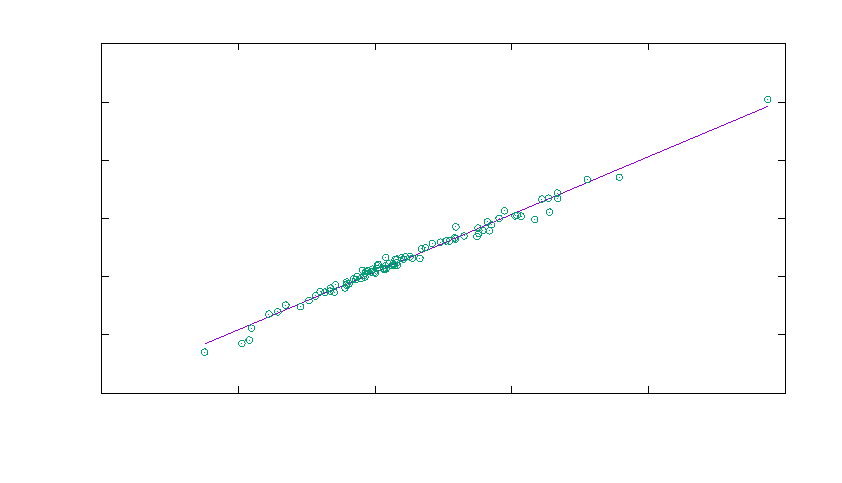
\includegraphics{../images/vehicle_corr}}%
    \gplfronttext
  \end{picture}%
\endgroup

%     }
%     \caption{Correlation between the two used ICAD instruments during
%       the Heidelberg vehicle measurement. The data points depict
%       \SI{1}{\minute} averages.}
%     \label{fig:flow}
%   \end{figure}
% \end{frame}

\begin{frame}
  \frametitle{Measurements}
  \framesubtitle{Vehicle Measurements}
  \begin{figure}[htbp]
    \centering
    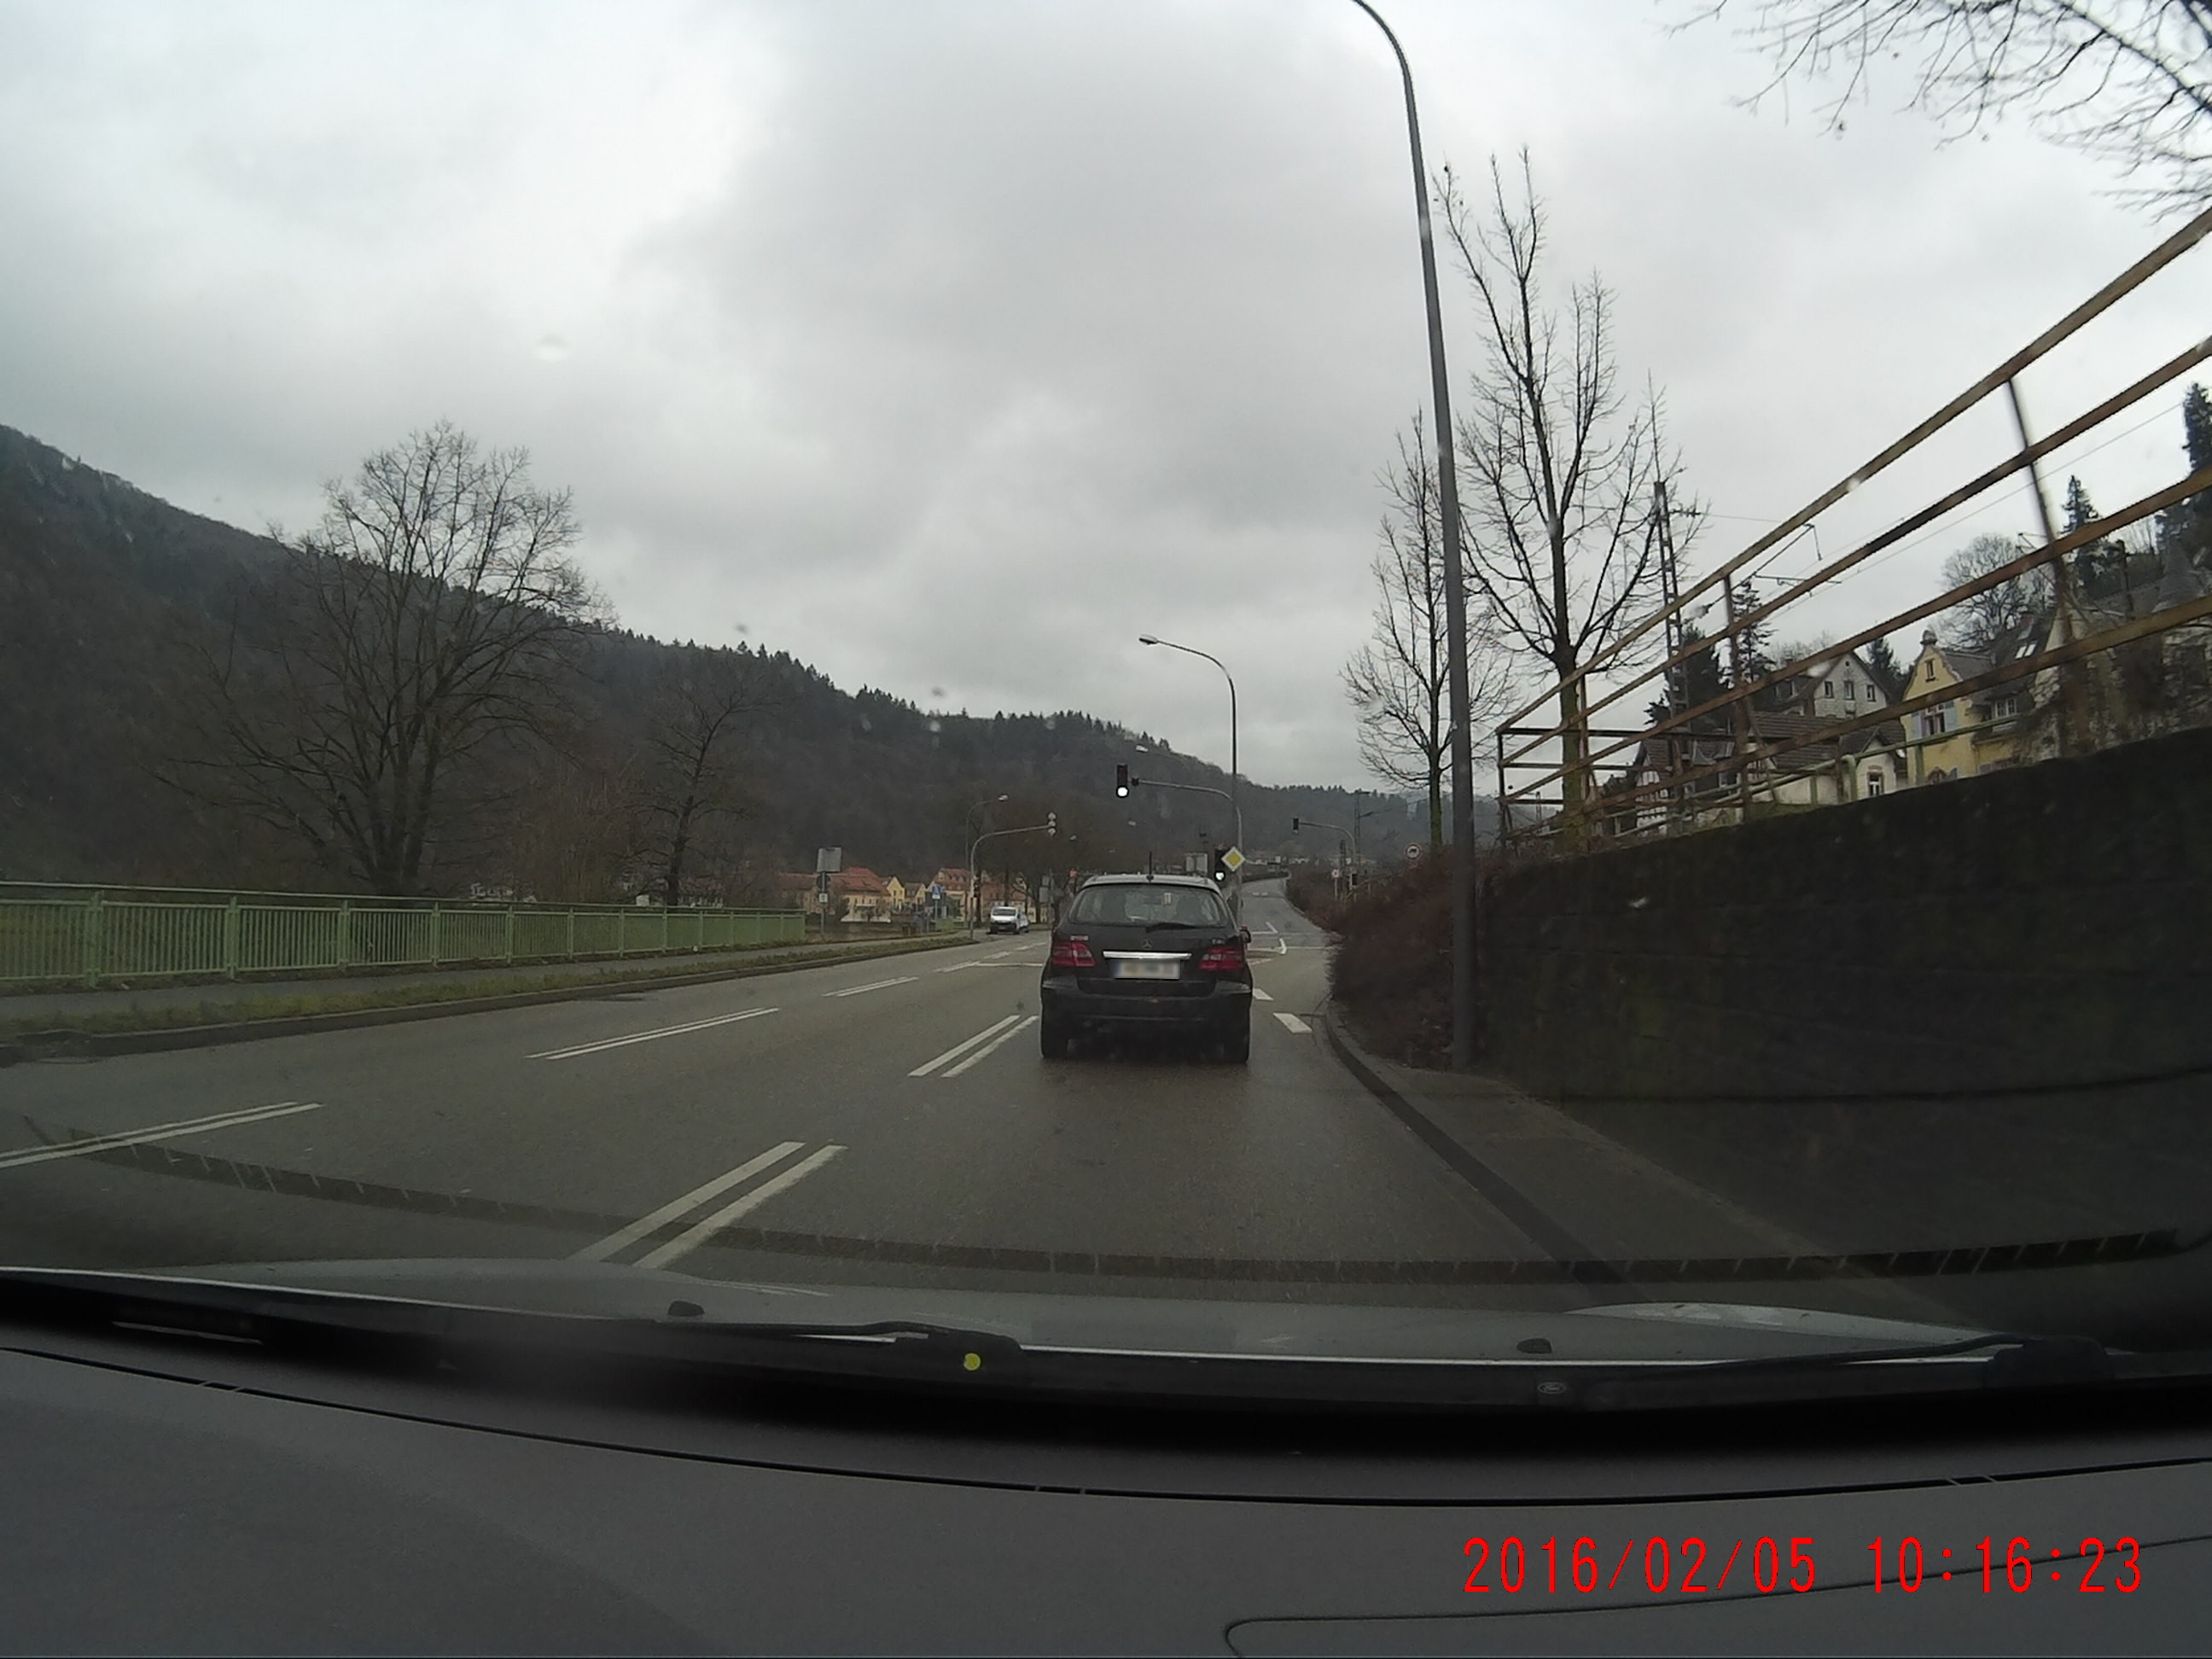
\includegraphics[width=0.45\textwidth]{mercedes.jpg}
    \hfill  
    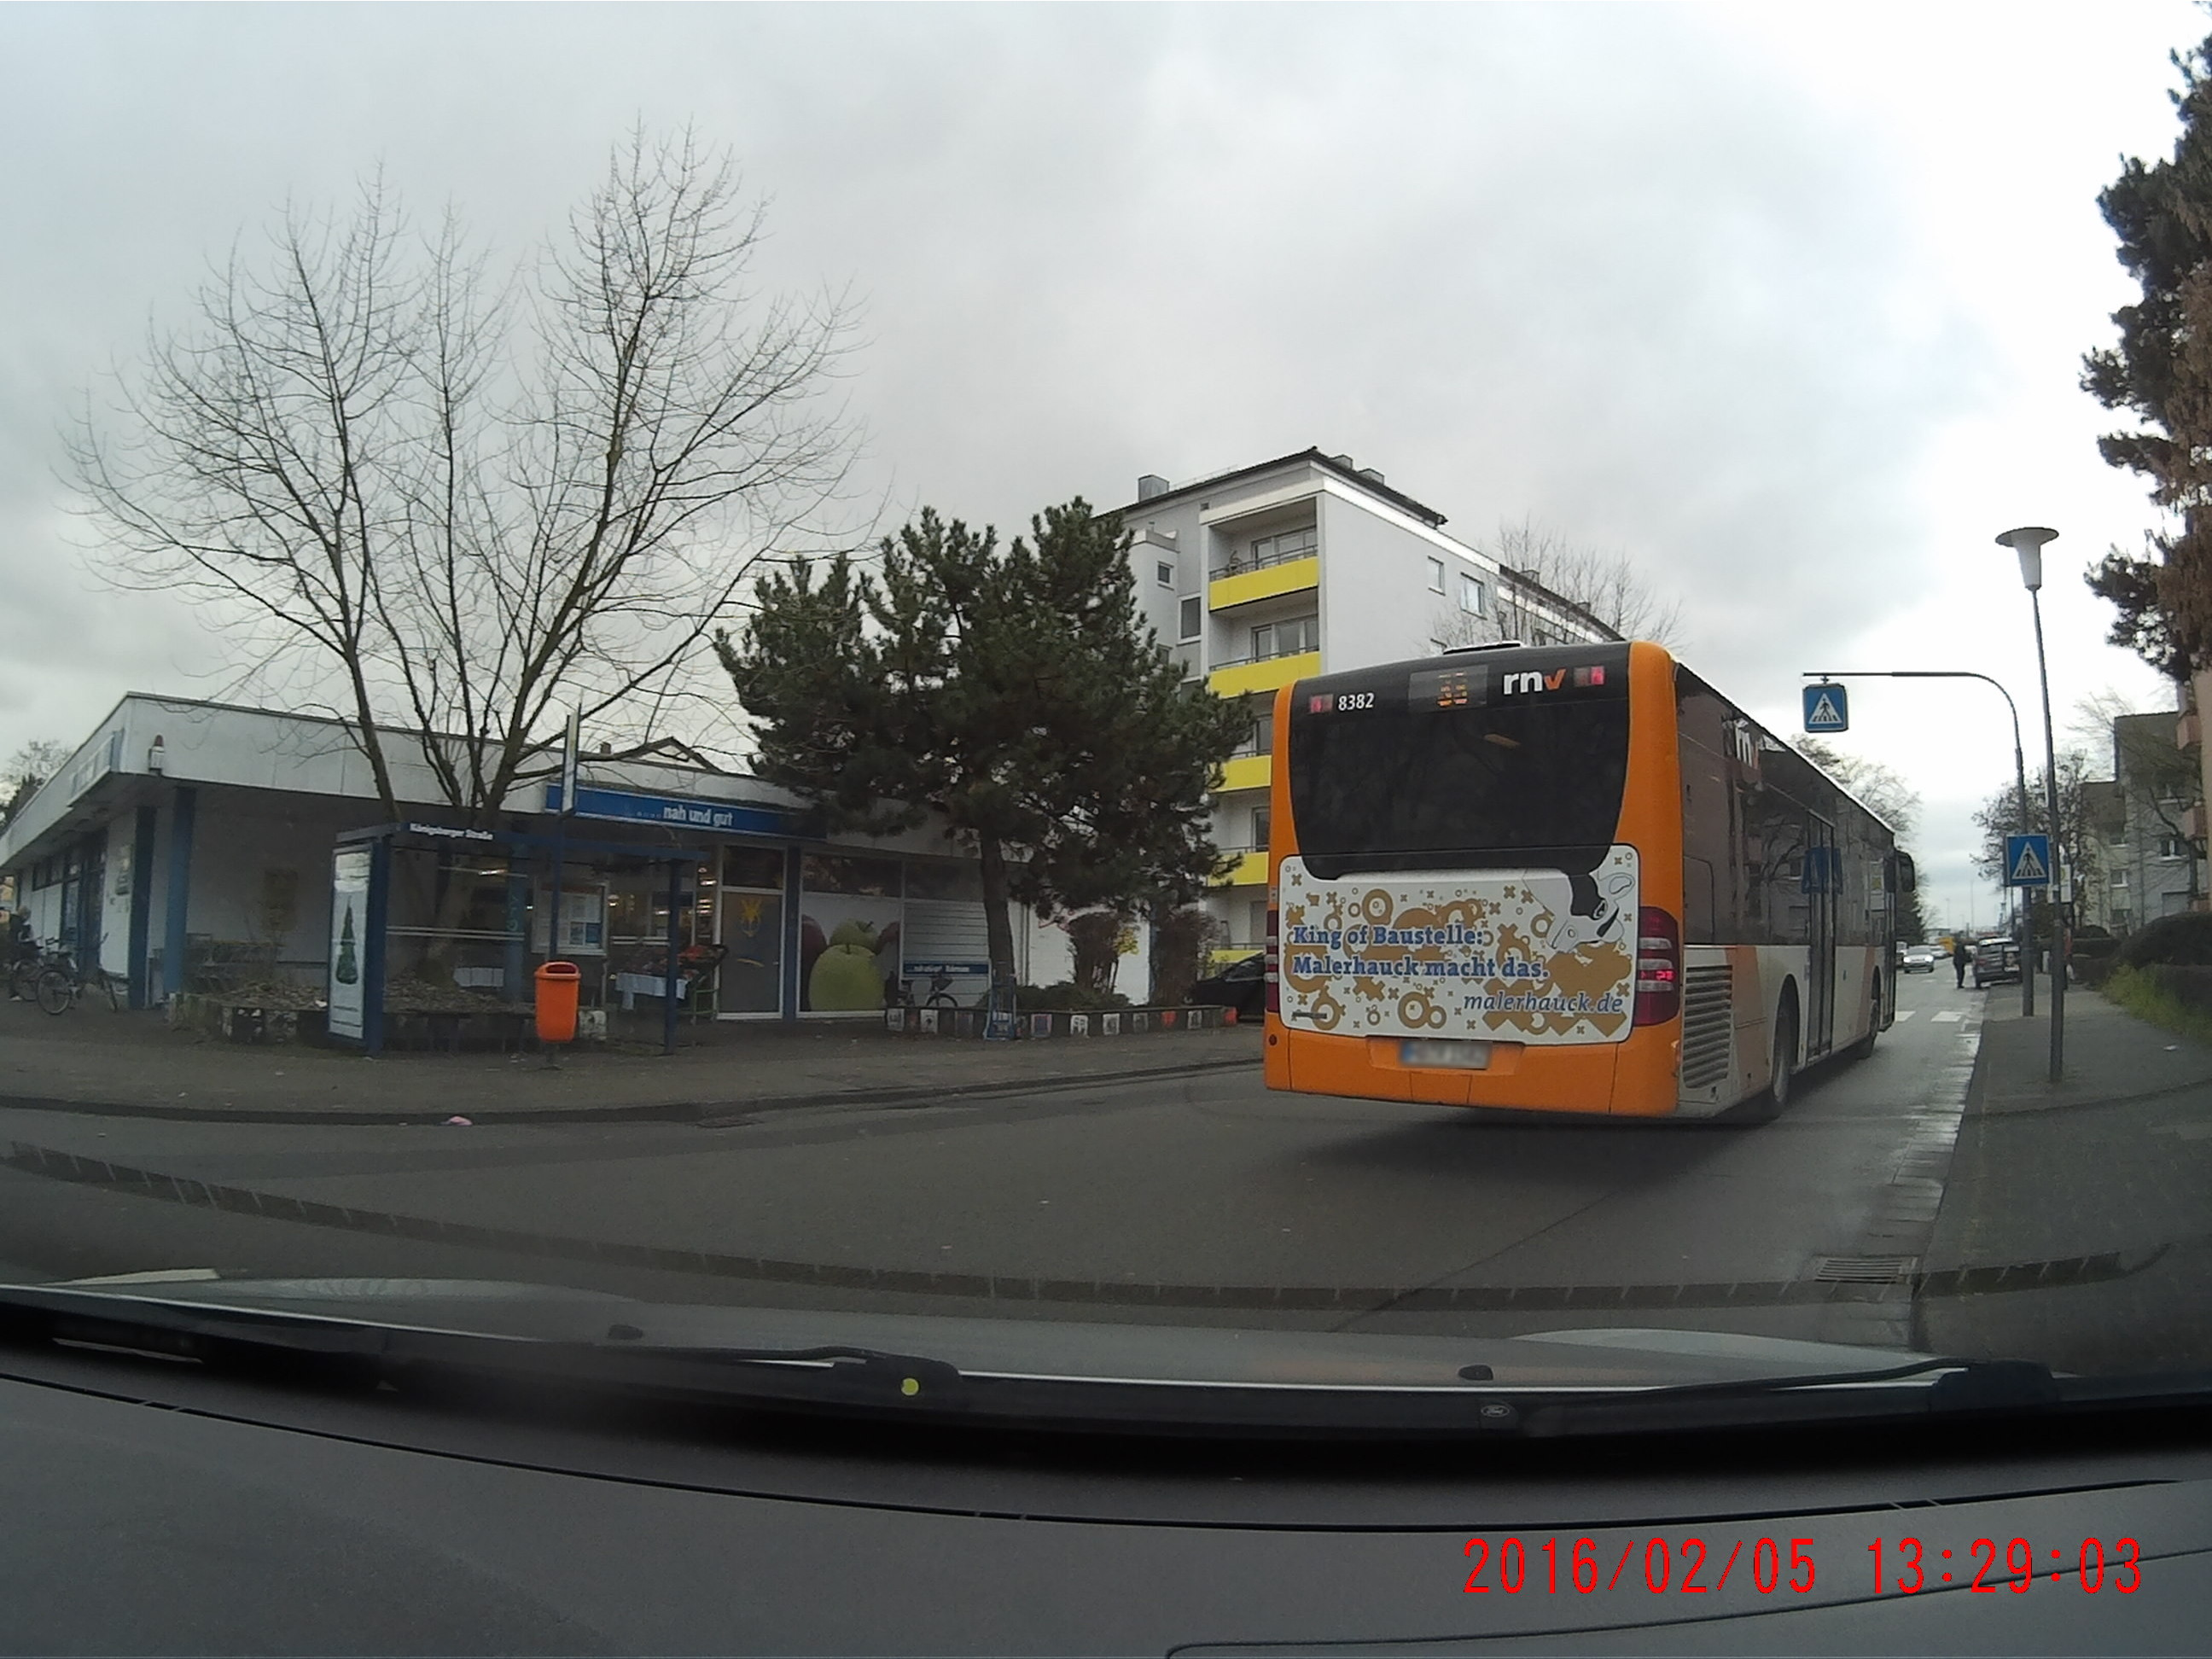
\includegraphics[width=0.45\textwidth]{bus.jpg}
    \caption{Picture of the measured bus and Mercedes B180 CDI. Please note that
      the printed time is in utc.}
    \label{fig:bus}
  \end{figure}
\end{frame}

\begin{frame}
  \frametitle{Measurements}
  \framesubtitle{Vehicle Measurements}
  \begin{figure}[htbp]
    \centering
    \scalebox{.42}{
      % GNUPLOT: LaTeX picture with Postscript
\begingroup
  \makeatletter
  \providecommand\color[2][]{%
    \GenericError{(gnuplot) \space\space\space\@spaces}{%
      Package color not loaded in conjunction with
      terminal option `colourtext'%
    }{See the gnuplot documentation for explanation.%
    }{Either use 'blacktext' in gnuplot or load the package
      color.sty in LaTeX.}%
    \renewcommand\color[2][]{}%
  }%
  \providecommand\includegraphics[2][]{%
    \GenericError{(gnuplot) \space\space\space\@spaces}{%
      Package graphicx or graphics not loaded%
    }{See the gnuplot documentation for explanation.%
    }{The gnuplot epslatex terminal needs graphicx.sty or graphics.sty.}%
    \renewcommand\includegraphics[2][]{}%
  }%
  \providecommand\rotatebox[2]{#2}%
  \@ifundefined{ifGPcolor}{%
    \newif\ifGPcolor
    \GPcolorfalse
  }{}%
  \@ifundefined{ifGPblacktext}{%
    \newif\ifGPblacktext
    \GPblacktexttrue
  }{}%
  % define a \g@addto@macro without @ in the name:
  \let\gplgaddtomacro\g@addto@macro
  % define empty templates for all commands taking text:
  \gdef\gplbacktext{}%
  \gdef\gplfronttext{}%
  \makeatother
  \ifGPblacktext
    % no textcolor at all
    \def\colorrgb#1{}%
    \def\colorgray#1{}%
  \else
    % gray or color?
    \ifGPcolor
      \def\colorrgb#1{\color[rgb]{#1}}%
      \def\colorgray#1{\color[gray]{#1}}%
      \expandafter\def\csname LTw\endcsname{\color{white}}%
      \expandafter\def\csname LTb\endcsname{\color{black}}%
      \expandafter\def\csname LTa\endcsname{\color{black}}%
      \expandafter\def\csname LT0\endcsname{\color[rgb]{1,0,0}}%
      \expandafter\def\csname LT1\endcsname{\color[rgb]{0,1,0}}%
      \expandafter\def\csname LT2\endcsname{\color[rgb]{0,0,1}}%
      \expandafter\def\csname LT3\endcsname{\color[rgb]{1,0,1}}%
      \expandafter\def\csname LT4\endcsname{\color[rgb]{0,1,1}}%
      \expandafter\def\csname LT5\endcsname{\color[rgb]{1,1,0}}%
      \expandafter\def\csname LT6\endcsname{\color[rgb]{0,0,0}}%
      \expandafter\def\csname LT7\endcsname{\color[rgb]{1,0.3,0}}%
      \expandafter\def\csname LT8\endcsname{\color[rgb]{0.5,0.5,0.5}}%
    \else
      % gray
      \def\colorrgb#1{\color{black}}%
      \def\colorgray#1{\color[gray]{#1}}%
      \expandafter\def\csname LTw\endcsname{\color{white}}%
      \expandafter\def\csname LTb\endcsname{\color{black}}%
      \expandafter\def\csname LTa\endcsname{\color{black}}%
      \expandafter\def\csname LT0\endcsname{\color{black}}%
      \expandafter\def\csname LT1\endcsname{\color{black}}%
      \expandafter\def\csname LT2\endcsname{\color{black}}%
      \expandafter\def\csname LT3\endcsname{\color{black}}%
      \expandafter\def\csname LT4\endcsname{\color{black}}%
      \expandafter\def\csname LT5\endcsname{\color{black}}%
      \expandafter\def\csname LT6\endcsname{\color{black}}%
      \expandafter\def\csname LT7\endcsname{\color{black}}%
      \expandafter\def\csname LT8\endcsname{\color{black}}%
    \fi
  \fi
    \setlength{\unitlength}{0.0500bp}%
    \ifx\gptboxheight\undefined%
      \newlength{\gptboxheight}%
      \newlength{\gptboxwidth}%
      \newsavebox{\gptboxtext}%
    \fi%
    \setlength{\fboxrule}{0.5pt}%
    \setlength{\fboxsep}{1pt}%
\begin{picture}(7200.00,5040.00)%
    \gplgaddtomacro\gplbacktext{%
      \csname LTb\endcsname%
      \put(946,966){\makebox(0,0)[r]{\strut{}$0$}}%
      \put(946,1347){\makebox(0,0)[r]{\strut{}$100$}}%
      \put(946,1728){\makebox(0,0)[r]{\strut{}$200$}}%
      \put(946,2109){\makebox(0,0)[r]{\strut{}$300$}}%
      \put(946,2490){\makebox(0,0)[r]{\strut{}$400$}}%
      \put(946,2871){\makebox(0,0)[r]{\strut{}$500$}}%
      \put(946,3251){\makebox(0,0)[r]{\strut{}$600$}}%
      \put(946,3632){\makebox(0,0)[r]{\strut{}$700$}}%
      \put(946,4013){\makebox(0,0)[r]{\strut{}$800$}}%
      \put(946,4394){\makebox(0,0)[r]{\strut{}$900$}}%
      \put(946,4775){\makebox(0,0)[r]{\strut{}$1000$}}%
      \put(1078,834){\rotatebox{-45}{\makebox(0,0)[l]{\strut{}11:15:00}}}%
      \put(1471,834){\rotatebox{-45}{\makebox(0,0)[l]{\strut{}11:15:30}}}%
      \put(1864,834){\rotatebox{-45}{\makebox(0,0)[l]{\strut{}11:16:00}}}%
      \put(2256,834){\rotatebox{-45}{\makebox(0,0)[l]{\strut{}11:16:30}}}%
      \put(2649,834){\rotatebox{-45}{\makebox(0,0)[l]{\strut{}11:17:00}}}%
      \put(3042,834){\rotatebox{-45}{\makebox(0,0)[l]{\strut{}11:17:30}}}%
      \put(3435,834){\rotatebox{-45}{\makebox(0,0)[l]{\strut{}11:18:00}}}%
      \put(3827,834){\rotatebox{-45}{\makebox(0,0)[l]{\strut{}11:18:30}}}%
      \put(4220,834){\rotatebox{-45}{\makebox(0,0)[l]{\strut{}11:19:00}}}%
      \put(4613,834){\rotatebox{-45}{\makebox(0,0)[l]{\strut{}11:19:30}}}%
      \put(5006,834){\rotatebox{-45}{\makebox(0,0)[l]{\strut{}11:20:00}}}%
      \put(5398,834){\rotatebox{-45}{\makebox(0,0)[l]{\strut{}11:20:30}}}%
      \put(5791,834){\rotatebox{-45}{\makebox(0,0)[l]{\strut{}11:21:00}}}%
      \put(5923,966){\makebox(0,0)[l]{\strut{}$0$}}%
      \put(5923,1347){\makebox(0,0)[l]{\strut{}$100$}}%
      \put(5923,1728){\makebox(0,0)[l]{\strut{}$200$}}%
      \put(5923,2109){\makebox(0,0)[l]{\strut{}$300$}}%
      \put(5923,2490){\makebox(0,0)[l]{\strut{}$400$}}%
      \put(5923,2871){\makebox(0,0)[l]{\strut{}$500$}}%
      \put(5923,3251){\makebox(0,0)[l]{\strut{}$600$}}%
      \put(5923,3632){\makebox(0,0)[l]{\strut{}$700$}}%
      \put(5923,4013){\makebox(0,0)[l]{\strut{}$800$}}%
      \put(5923,4394){\makebox(0,0)[l]{\strut{}$900$}}%
      \put(5923,4775){\makebox(0,0)[l]{\strut{}$1000$}}%
    }%
    \gplgaddtomacro\gplfronttext{%
      \csname LTb\endcsname%
      \put(176,2870){\rotatebox{-270}{\makebox(0,0){\strut{}\ch{NO2}/\ch{NO_x} Concentration [ppb]}}}%
      \put(6692,2870){\rotatebox{-270}{\makebox(0,0){\strut{}\ch{CO2} Concentration [ppm]}}}%
      \csname LTb\endcsname%
      \put(4804,4602){\makebox(0,0)[r]{\strut{}\ch{NO2}}}%
      \csname LTb\endcsname%
      \put(4804,4382){\makebox(0,0)[r]{\strut{}\ch{NO_x}}}%
      \csname LTb\endcsname%
      \put(4804,4162){\makebox(0,0)[r]{\strut{}\ch{CO2}}}%
    }%
    \gplbacktext
    \put(0,0){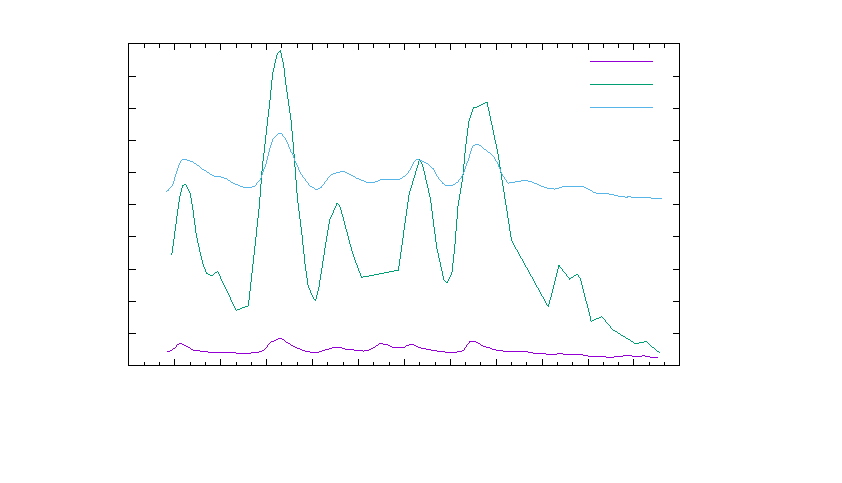
\includegraphics{../images/mercedes}}%
    \gplfronttext
  \end{picture}%
\endgroup

    }
    \hfill
    \scalebox{.42}{
      % GNUPLOT: LaTeX picture with Postscript
\begingroup
  \makeatletter
  \providecommand\color[2][]{%
    \GenericError{(gnuplot) \space\space\space\@spaces}{%
      Package color not loaded in conjunction with
      terminal option `colourtext'%
    }{See the gnuplot documentation for explanation.%
    }{Either use 'blacktext' in gnuplot or load the package
      color.sty in LaTeX.}%
    \renewcommand\color[2][]{}%
  }%
  \providecommand\includegraphics[2][]{%
    \GenericError{(gnuplot) \space\space\space\@spaces}{%
      Package graphicx or graphics not loaded%
    }{See the gnuplot documentation for explanation.%
    }{The gnuplot epslatex terminal needs graphicx.sty or graphics.sty.}%
    \renewcommand\includegraphics[2][]{}%
  }%
  \providecommand\rotatebox[2]{#2}%
  \@ifundefined{ifGPcolor}{%
    \newif\ifGPcolor
    \GPcolorfalse
  }{}%
  \@ifundefined{ifGPblacktext}{%
    \newif\ifGPblacktext
    \GPblacktexttrue
  }{}%
  % define a \g@addto@macro without @ in the name:
  \let\gplgaddtomacro\g@addto@macro
  % define empty templates for all commands taking text:
  \gdef\gplbacktext{}%
  \gdef\gplfronttext{}%
  \makeatother
  \ifGPblacktext
    % no textcolor at all
    \def\colorrgb#1{}%
    \def\colorgray#1{}%
  \else
    % gray or color?
    \ifGPcolor
      \def\colorrgb#1{\color[rgb]{#1}}%
      \def\colorgray#1{\color[gray]{#1}}%
      \expandafter\def\csname LTw\endcsname{\color{white}}%
      \expandafter\def\csname LTb\endcsname{\color{black}}%
      \expandafter\def\csname LTa\endcsname{\color{black}}%
      \expandafter\def\csname LT0\endcsname{\color[rgb]{1,0,0}}%
      \expandafter\def\csname LT1\endcsname{\color[rgb]{0,1,0}}%
      \expandafter\def\csname LT2\endcsname{\color[rgb]{0,0,1}}%
      \expandafter\def\csname LT3\endcsname{\color[rgb]{1,0,1}}%
      \expandafter\def\csname LT4\endcsname{\color[rgb]{0,1,1}}%
      \expandafter\def\csname LT5\endcsname{\color[rgb]{1,1,0}}%
      \expandafter\def\csname LT6\endcsname{\color[rgb]{0,0,0}}%
      \expandafter\def\csname LT7\endcsname{\color[rgb]{1,0.3,0}}%
      \expandafter\def\csname LT8\endcsname{\color[rgb]{0.5,0.5,0.5}}%
    \else
      % gray
      \def\colorrgb#1{\color{black}}%
      \def\colorgray#1{\color[gray]{#1}}%
      \expandafter\def\csname LTw\endcsname{\color{white}}%
      \expandafter\def\csname LTb\endcsname{\color{black}}%
      \expandafter\def\csname LTa\endcsname{\color{black}}%
      \expandafter\def\csname LT0\endcsname{\color{black}}%
      \expandafter\def\csname LT1\endcsname{\color{black}}%
      \expandafter\def\csname LT2\endcsname{\color{black}}%
      \expandafter\def\csname LT3\endcsname{\color{black}}%
      \expandafter\def\csname LT4\endcsname{\color{black}}%
      \expandafter\def\csname LT5\endcsname{\color{black}}%
      \expandafter\def\csname LT6\endcsname{\color{black}}%
      \expandafter\def\csname LT7\endcsname{\color{black}}%
      \expandafter\def\csname LT8\endcsname{\color{black}}%
    \fi
  \fi
    \setlength{\unitlength}{0.0500bp}%
    \ifx\gptboxheight\undefined%
      \newlength{\gptboxheight}%
      \newlength{\gptboxwidth}%
      \newsavebox{\gptboxtext}%
    \fi%
    \setlength{\fboxrule}{0.5pt}%
    \setlength{\fboxsep}{1pt}%
\begin{picture}(7200.00,5040.00)%
    \gplgaddtomacro\gplbacktext{%
      \csname LTb\endcsname%
      \put(946,966){\makebox(0,0)[r]{\strut{}$0$}}%
      \put(946,1389){\makebox(0,0)[r]{\strut{}$500$}}%
      \put(946,1812){\makebox(0,0)[r]{\strut{}$1000$}}%
      \put(946,2236){\makebox(0,0)[r]{\strut{}$1500$}}%
      \put(946,2659){\makebox(0,0)[r]{\strut{}$2000$}}%
      \put(946,3082){\makebox(0,0)[r]{\strut{}$2500$}}%
      \put(946,3505){\makebox(0,0)[r]{\strut{}$3000$}}%
      \put(946,3929){\makebox(0,0)[r]{\strut{}$3500$}}%
      \put(946,4352){\makebox(0,0)[r]{\strut{}$4000$}}%
      \put(946,4775){\makebox(0,0)[r]{\strut{}$4500$}}%
      \put(1078,834){\rotatebox{-45}{\makebox(0,0)[l]{\strut{}14:25:00}}}%
      \put(1549,834){\rotatebox{-45}{\makebox(0,0)[l]{\strut{}14:26:00}}}%
      \put(2021,834){\rotatebox{-45}{\makebox(0,0)[l]{\strut{}14:27:00}}}%
      \put(2492,834){\rotatebox{-45}{\makebox(0,0)[l]{\strut{}14:28:00}}}%
      \put(2963,834){\rotatebox{-45}{\makebox(0,0)[l]{\strut{}14:29:00}}}%
      \put(3435,834){\rotatebox{-45}{\makebox(0,0)[l]{\strut{}14:30:00}}}%
      \put(3906,834){\rotatebox{-45}{\makebox(0,0)[l]{\strut{}14:31:00}}}%
      \put(4377,834){\rotatebox{-45}{\makebox(0,0)[l]{\strut{}14:32:00}}}%
      \put(4848,834){\rotatebox{-45}{\makebox(0,0)[l]{\strut{}14:33:00}}}%
      \put(5320,834){\rotatebox{-45}{\makebox(0,0)[l]{\strut{}14:34:00}}}%
      \put(5791,834){\rotatebox{-45}{\makebox(0,0)[l]{\strut{}14:35:00}}}%
      \put(5923,966){\makebox(0,0)[l]{\strut{}$0$}}%
      \put(5923,1389){\makebox(0,0)[l]{\strut{}$500$}}%
      \put(5923,1812){\makebox(0,0)[l]{\strut{}$1000$}}%
      \put(5923,2236){\makebox(0,0)[l]{\strut{}$1500$}}%
      \put(5923,2659){\makebox(0,0)[l]{\strut{}$2000$}}%
      \put(5923,3082){\makebox(0,0)[l]{\strut{}$2500$}}%
      \put(5923,3505){\makebox(0,0)[l]{\strut{}$3000$}}%
      \put(5923,3929){\makebox(0,0)[l]{\strut{}$3500$}}%
      \put(5923,4352){\makebox(0,0)[l]{\strut{}$4000$}}%
      \put(5923,4775){\makebox(0,0)[l]{\strut{}$4500$}}%
    }%
    \gplgaddtomacro\gplfronttext{%
      \csname LTb\endcsname%
      \put(176,2870){\rotatebox{-270}{\makebox(0,0){\strut{}\ch{NO2}/\ch{NO_x} Concentration [ppb]}}}%
      \put(6692,2870){\rotatebox{-270}{\makebox(0,0){\strut{}\ch{CO2} Concentration [ppm]}}}%
      \csname LTb\endcsname%
      \put(1738,4602){\makebox(0,0)[r]{\strut{}\ch{NO2}}}%
      \csname LTb\endcsname%
      \put(1738,4382){\makebox(0,0)[r]{\strut{}\ch{NO_x}}}%
      \csname LTb\endcsname%
      \put(1738,4162){\makebox(0,0)[r]{\strut{}\ch{CO2}}}%
    }%
    \gplbacktext
    \put(0,0){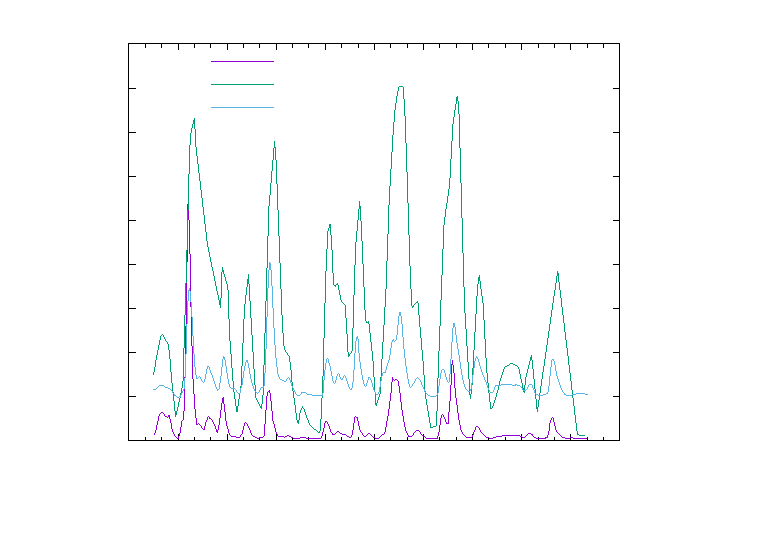
\includegraphics{../images/bus}}%
    \gplfronttext
  \end{picture}%
\endgroup

    }
    \caption{Time series of the uncorrected \ch{NO2}, \ch{NO_x} and
      \ch{CO2} concentrations in the plume of a Mercedes B180 CDI and
      a bus.}
    \label{fig:mercedes-ts}
  \end{figure}
  \begin{itemize}
  \item \ch{NO} saturation effects might have to be considered
  \end{itemize}
\end{frame}

% \begin{frame}
%   \frametitle{Measurements}
%   \framesubtitle{Vehicle Measurements}

%   \begin{table}[hbtp]
%     \sisetup{table-auto-round}
%     \centering
%     \scalebox{.8}{
%       \begin{tabular}{lS[table-format=1.1(1)e-1]
%         S[table-format=1.3(1)]
%         S[table-format=1.1(1)e-1]
%         S[table-format=1.2(1)]
%         }
%         \toprule
%         & {\ch{NO2}/\ch{CO2}} & {\ch{NO2} emission} & {\ch{NO_x}/\ch{CO2}} &
%                                                                              {\ch{NO_x}
%                                                                              emission}\\
%         & & {\si{\gram\per\kilo\meter}} & & {\si{\gram\per\kilo\meter}}\\
%         \midrule
%         Mercedes & 2.2(3)e-4 & 0.034(5) & 5.0(7)e-3 & 0.53(7)\\
%         Bus &  6(2)e-4 & 0.7(2) & 6(1)e-3 & 4.6(8)\\
%         \bottomrule
%       \end{tabular}
%     }
%     \caption{\ch{NO2} and \ch{NO_x} to \ch{CO2} ratios together with the
%       extrapolated emissions for the two vehicles.}
%     \label{tab:mercedes-bus}
%   \end{table}
% \end{frame}

\begin{frame}
  \frametitle{Conclusion \& Outlook}
  \begin{itemize}
  \item Silica gel filter in Ozone generator works
  \item Pure \ch{NO} measurements work
  \item \ch{NO_x} vehicle measurements work
    \begin{itemize}
    \item Ozone flow increase should be considered
    \end{itemize}
  \item Alternating measurement mode needs more work
    \begin{itemize}
    \item Ozone concentration decays slowly
    \item Adsorption at tube walls should be researched
    \item Alternatively, two ICAD cells can be used
    \end{itemize}
  \end{itemize}
\end{frame}

\begin{frame}
  \frametitle{Thank you}
  \centering
  Further questions?
\end{frame}

\nocite{*}
\begin{frame}
  \frametitle{Bibliography}
  \framesubtitle{Extract}
  \printbibliography{}
\end{frame}

\end{document}